\chapter{Results and discussion}

\section{Final dataset composition}

\begin{figure}[ht]
    \centering
    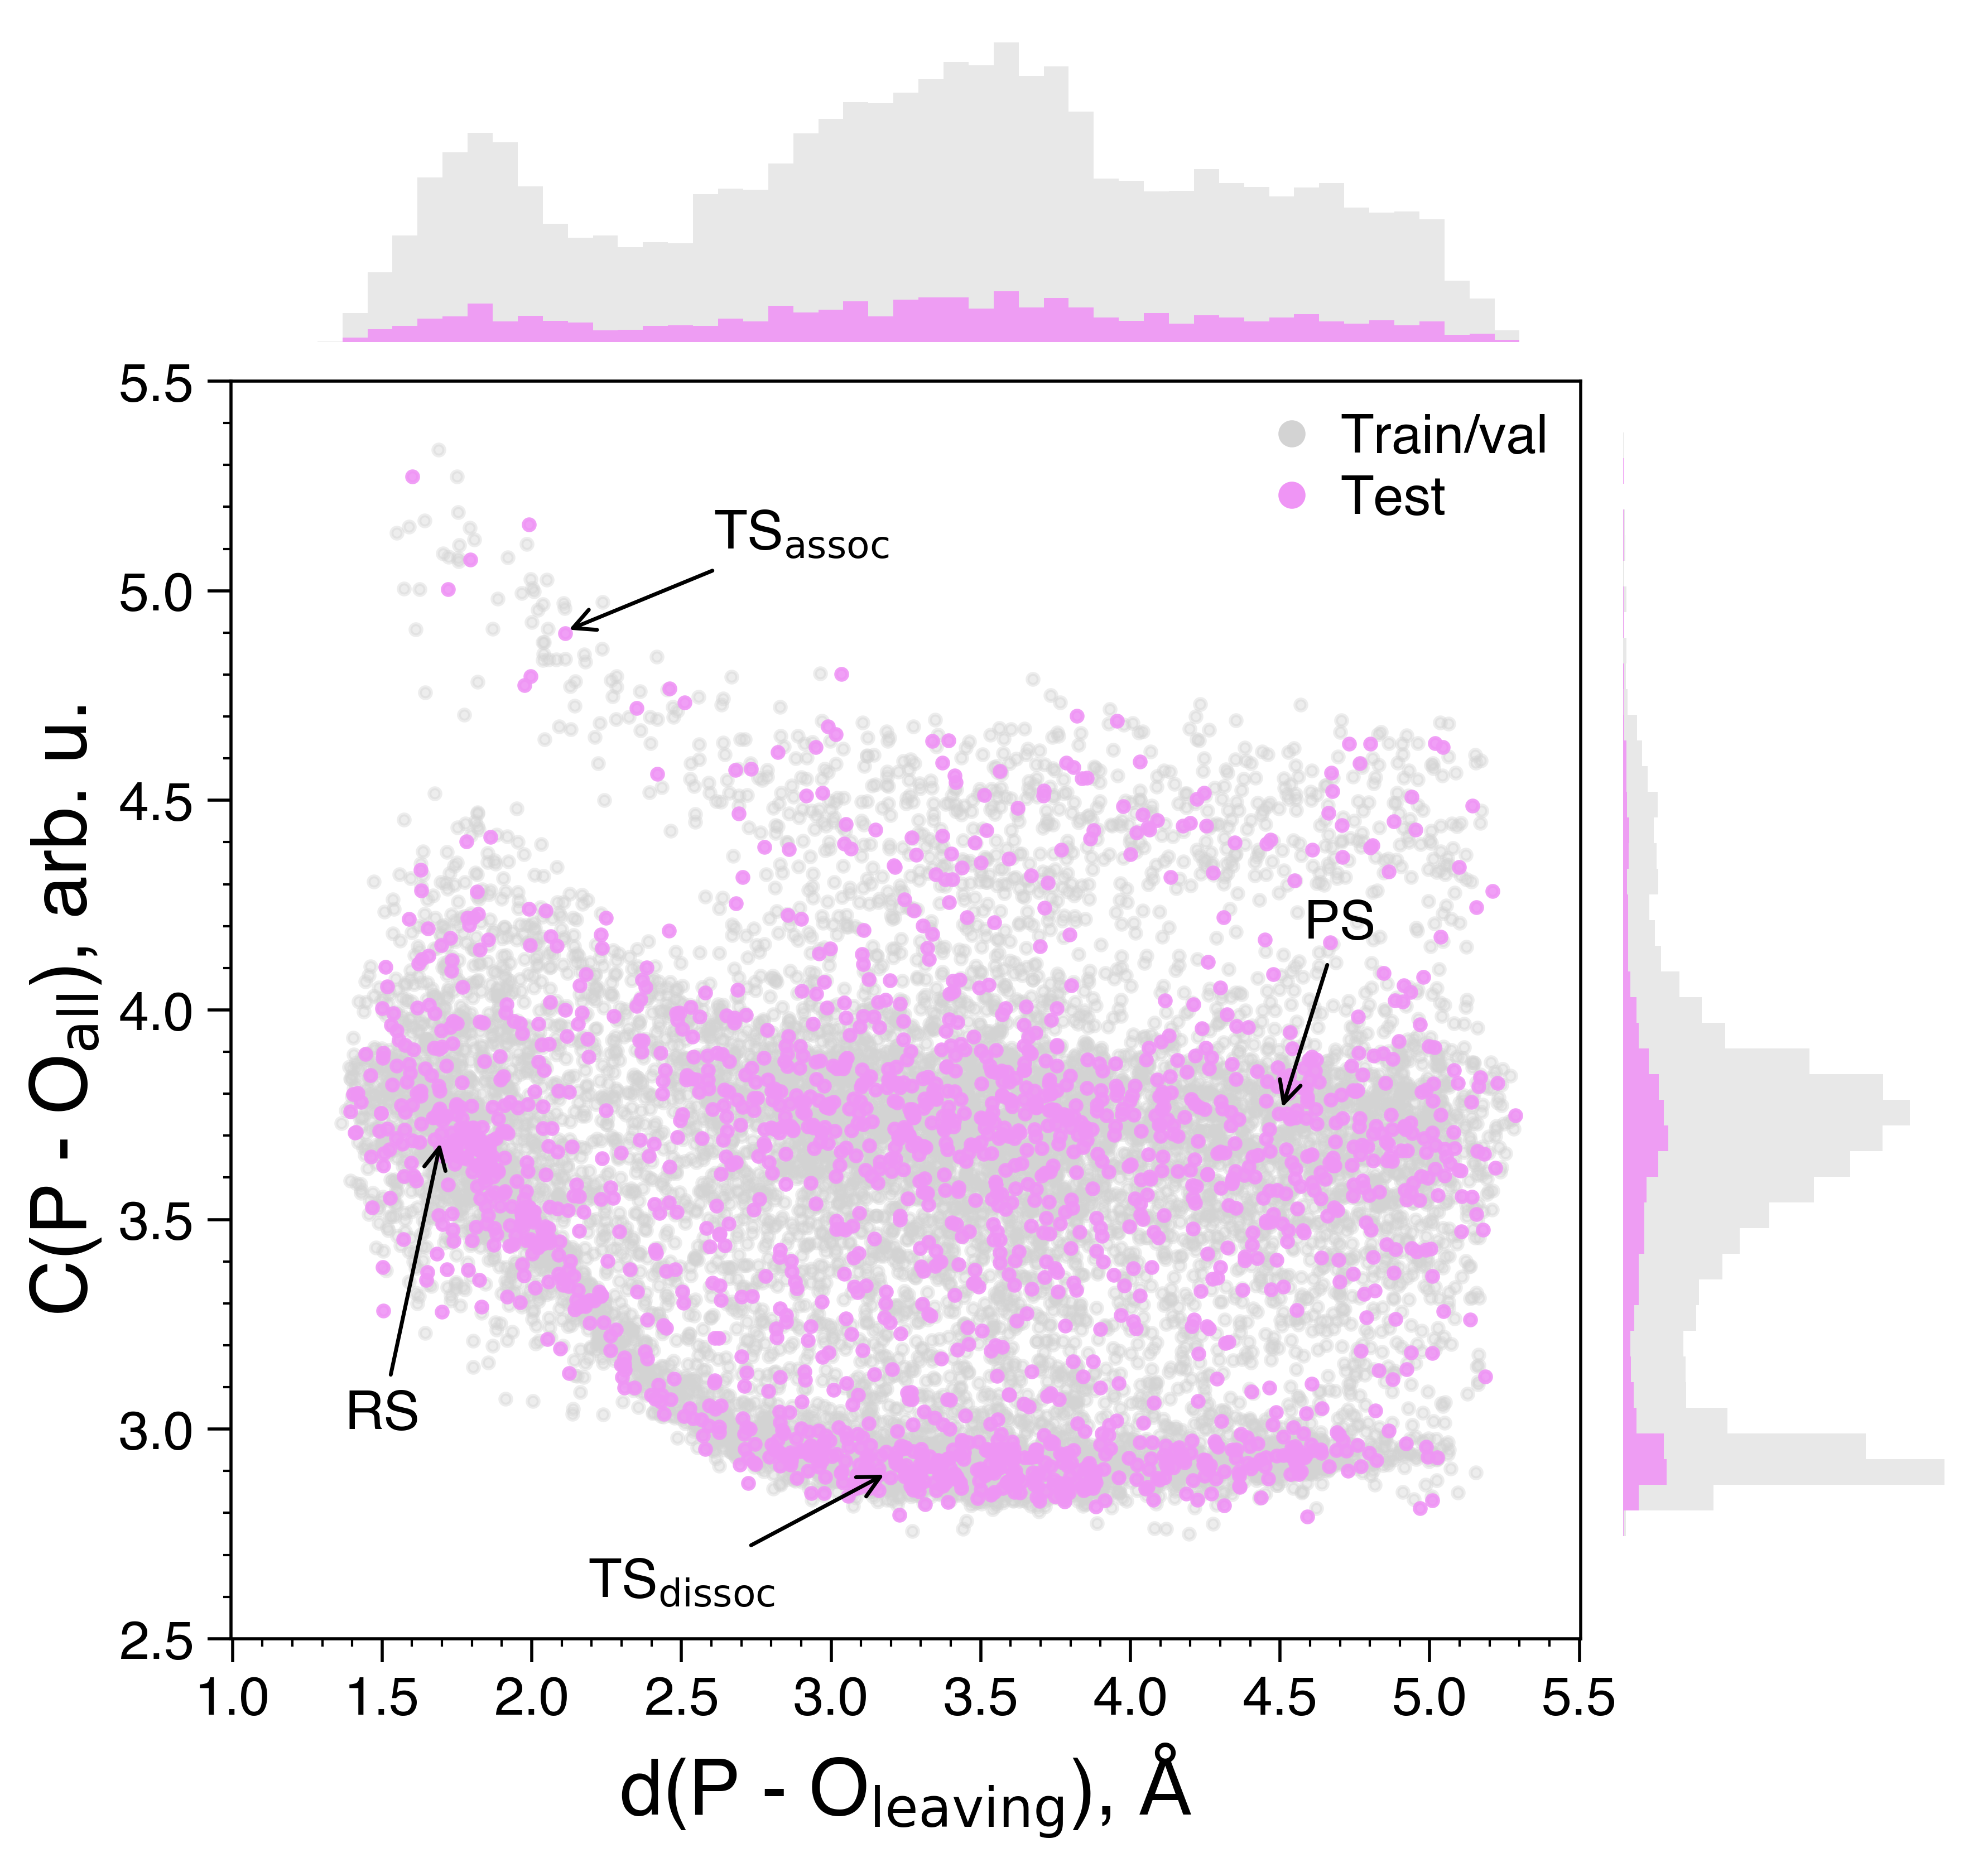
\includegraphics[width=0.9\textwidth]{Figures/4_Results/results_final_dataset_with_histograms.png}
    \caption{Left panel: final dataset composition projected on the two \acp{cv} space. RS stands for the reactant state, PS for the product state, and TS for the transition state. 50 bins were used to produce the histograms. Right panel: normalised densities of the two \acp{cv} for the training/validation and test sets.}
    \label{fig:final_dataset}
\end{figure}

The final dataset was obtained after three iterations of a learning loop, as described in Section~\ref{subsec:iterative-training-of-the-neural-network-potential}. During each iteration, the dataset was expanded by adding points from different regions of the \ac{fes}. This was achieved by imposing constraints on the \acp{cv}. For instance, in the first iteration, sampling primarily targeted the reactant and product basins, while in the second iteration, the focus shifted towards the transition state regions. The final iteration was dedicated to exploring the \ac{fes} at elevated temperatures (e.g., 320 and 340~K) in order to enhance the configurational diversity of the dataset. Sampling at higher temperatures generally improves the \ac{cv} space coverage, as it allows the system to visit higher-energy regions.

The final dataset comprises 12,000 data points for the training and validation sets, and 1,800 points for the test set, as illustrated in the left panel of Figure~\ref{fig:final_dataset}.

The reactant basin is well-defined, appearing as a narrow region in the \ac{cv} space. In contrast, the product basin is broader due to the diffusion of products within the simulation cell.

The sampling quality of the \ac{ts} regions varies. The dissociative pathway is substantially better represented than the associative one. This difference arises from the fact that the associative path lies higher in energy and is therefore more difficult to access. Nevertheless, it is still represented by a number of points, meaning the fitted potential should be capable of describing it to some extent.

A particularly important aspect of dataset construction was the implementation of density-aware sampling. This approach was adopted for several reasons. First and foremost, the algorithm was used to ensure that the dataset is balanced in terms of the \acp{cv} distribution, as shown in the right panel of Figure~\ref{fig:final_dataset}. Secondly, it was employed to guarantee sufficient configurational diversity, i.e., the inclusion of points from various physically meaningful regions of the \ac{fes}, thereby enhancing the potential's ability to generalise. This is crucial, as the neural network potential must be capable of predicting energies and forces for any configuration along the reaction coordinate. Lastly, density-aware sampling was used to ensure that the test set reflects the overall reaction space well, thereby providing a reliable basis for critically evaluating the accuracy and performance of the trained potential.



%%%%%%%%%%%%%%%%%%%%%%%%%%%%%%%%%%%%%%%%%%%%%%%%%%%%%%%%%%%%%%%%%%%%%%%%%%%%%%%%
\section{Accuracy and performance of the neural network potential}

\begin{figure}[t]
    \centering
    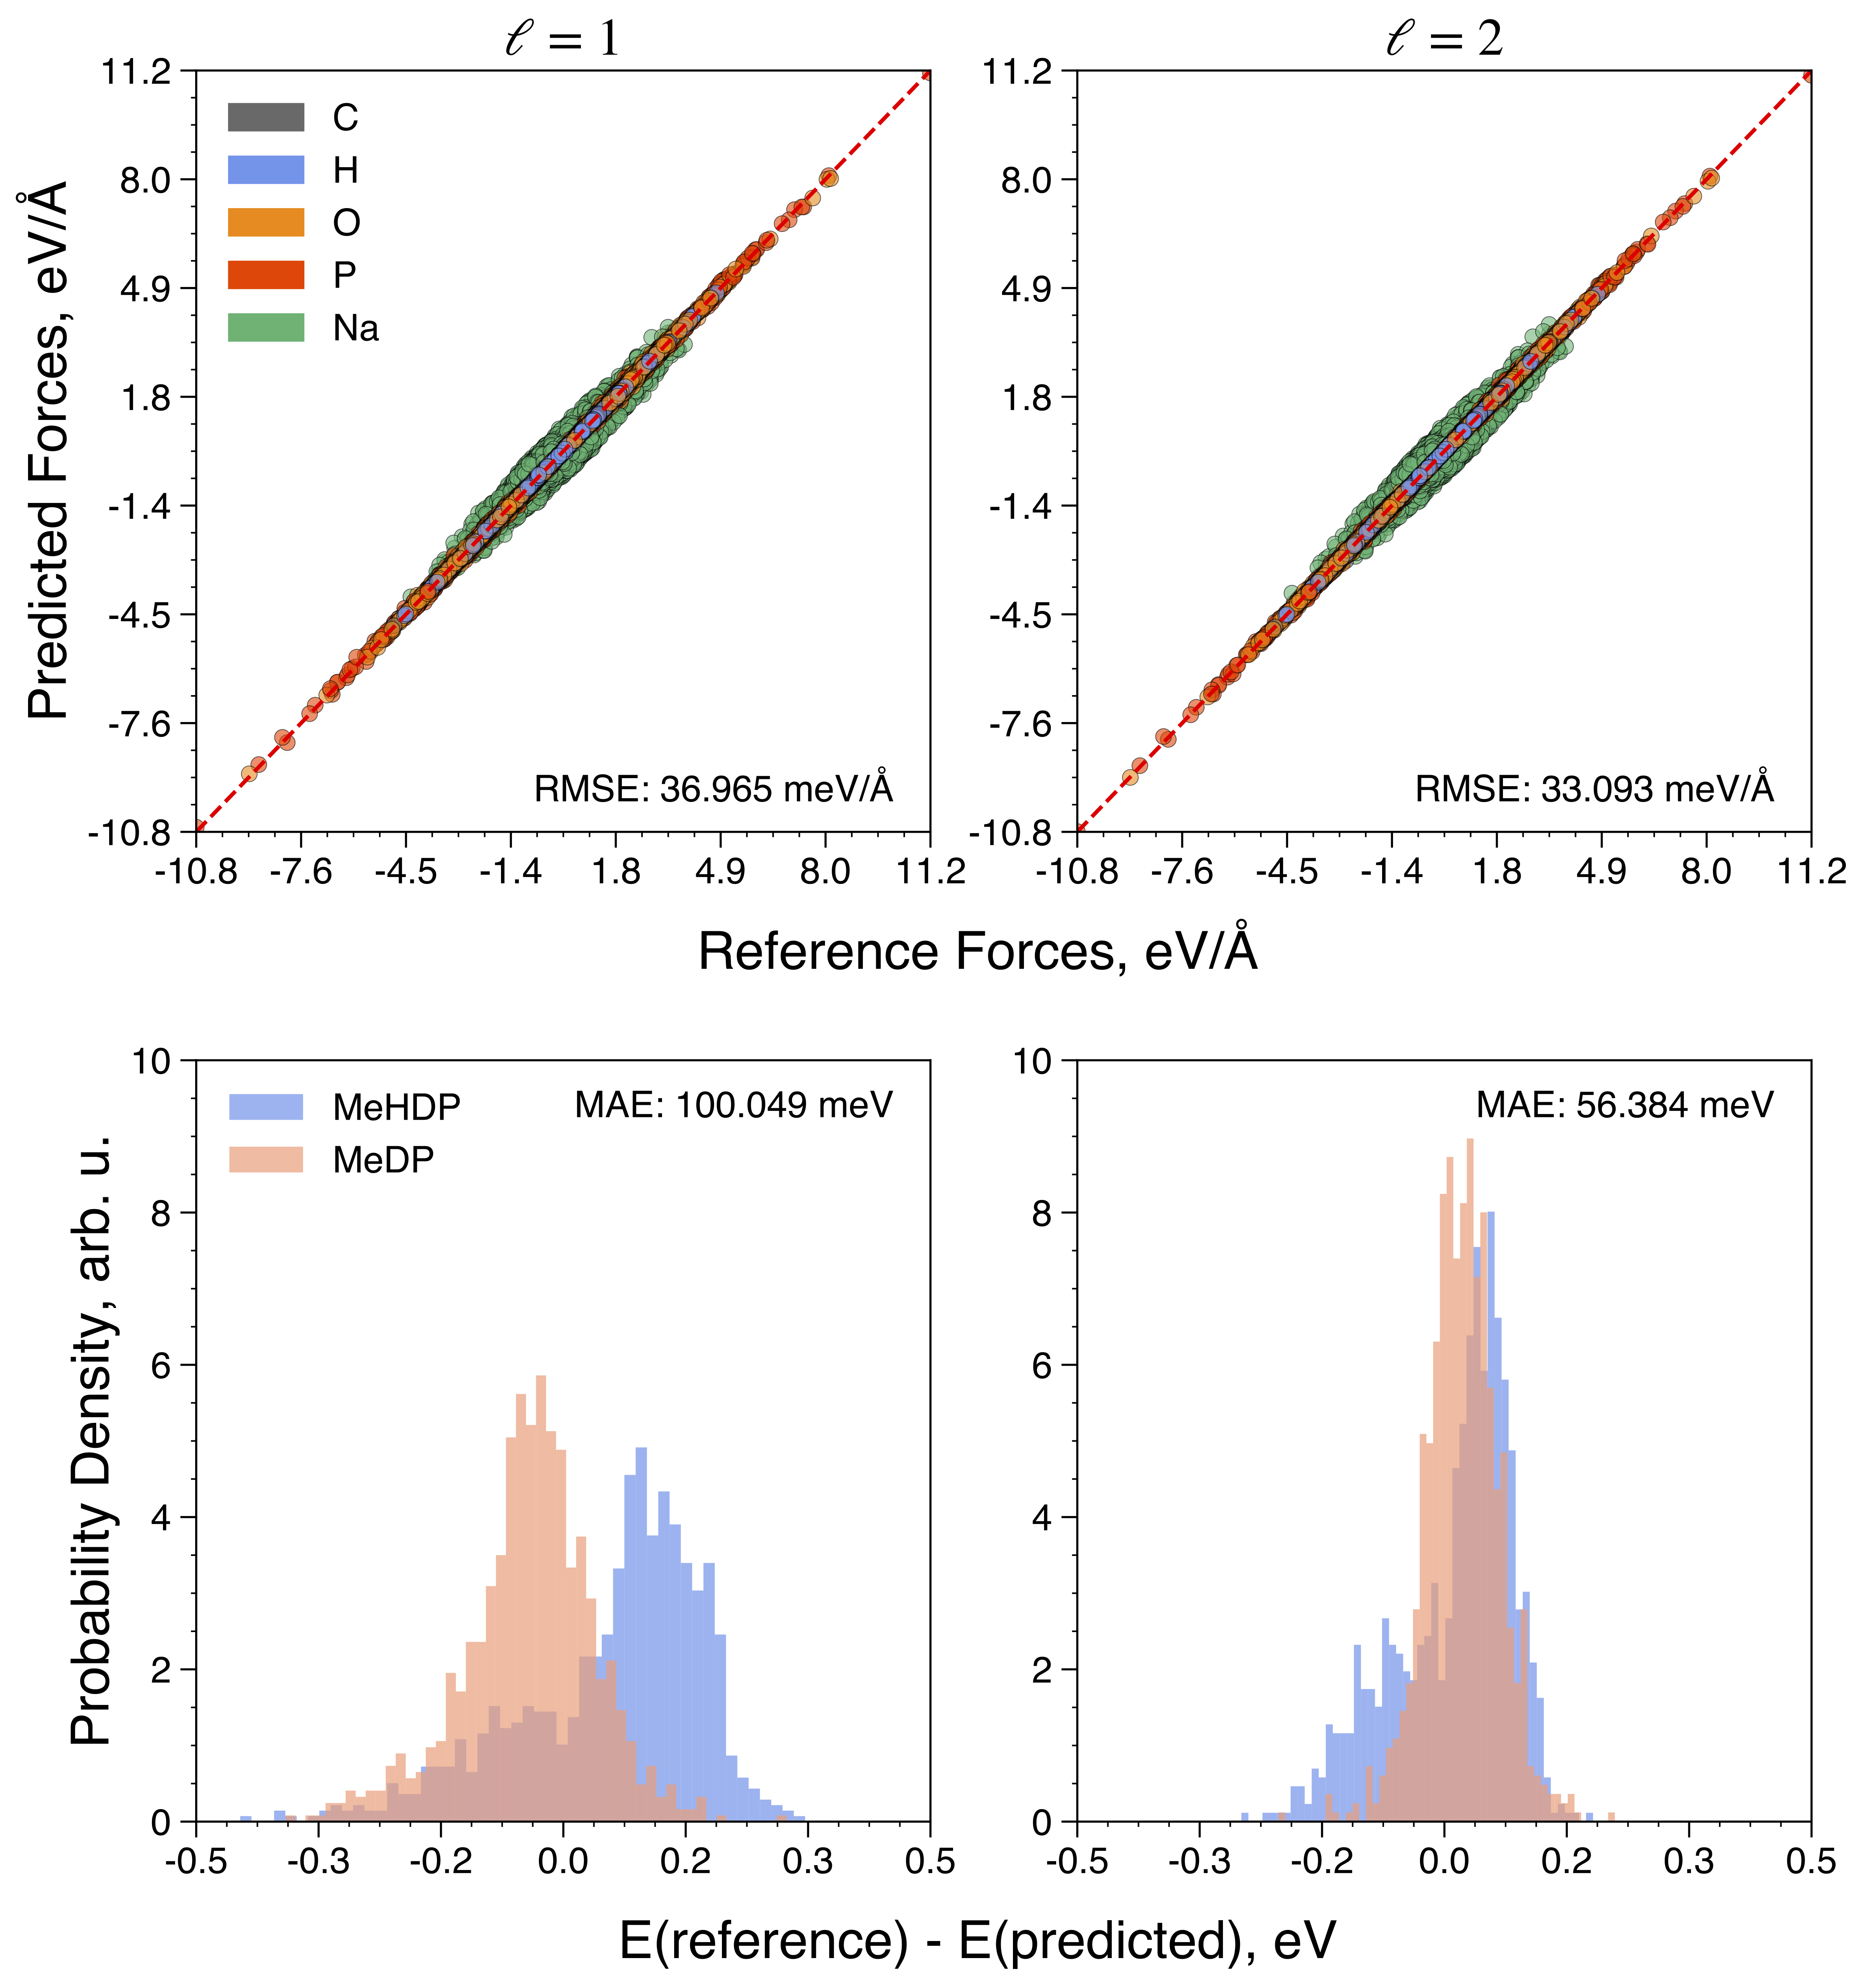
\includegraphics[width=0.8\textwidth]{Figures/4_Results/results_nnp_accuracy_l-1_l-2.png}
    \caption{Accuracy of the neural network potential trained on 12,000 data points. The left panel shows the errors in the forces and energy for the tensor rank $\ell=1$, and the right panel shows the errors for $\ell=2$. For the histograms, the number of bins was set to 50.}
    \label{fig:nnp_accuracy}
\end{figure}

At each iteration, the potential was fitted using a NequIP equivariant \ac{gnn} with a different tensor rank~$\ell$, namely $\ell=1$ and $\ell=2$ ($\ell=0$ would correspond to an invariant \ac{gnn}). The reason for using different tensor ranks was to investigate how the network complexity affects the accuracy of the potential. The tensor rank $\ell$ determines the number of parameters in the network, with higher values leading to more complex node representations.

The final potential was trained on 12,000 data points, and its accuracy is illustrated in Figure~\ref{fig:nnp_accuracy}. The left panel shows the errors in the forces and energy for tensor rank $\ell=1$, while the right panel shows the corresponding errors for $\ell=2$. The errors are calculated as the difference between the neural network potential and the reference \ac{dft} values.

According to current community standards~\citep{jacobsPracticalGuideMachine2025a}, the accuracy of a neural network potential is considered a `very good fit' when the \ac{rmse} in the forces lies within the range of 20-40~meV/\AA\ and the \ac{mae} in the energy is between 1-10~meV/atom. A `very accurate fit' is defined as the \ac{rmse} in the forces of approximately 10~meV/\AA\ and the \ac{mae} in the energy on the order of 1~meV/atom.

The \acp{nnp} obtained in this work fall somewhere in between these two categories. The \ac{rmse} in the forces is 37.069~meV/\AA\ for $\ell=1$ and 33.142~meV/\AA\ for $\ell=2$, while the \ac{mae} in the energy is below 0.3~meV/atom for $\ell=1$ and below 0.15~meV/atom for $\ell=2$.

As shown in Figure~\ref{fig:nnp_accuracy}, the errors in the forces lie along the diagonal, which represents a perfect fit. The only points that are slightly scattered correspond to sodium cations (Na\textsuperscript{+}) jiggling in solution, not being technically bound to anything. This makes it more challenging for the network to predict the forces on them.

Regarding the energy predictions, the potential with $\ell=1$ slightly overestimates them. This can be seen from the tail of the probability density on the left-hand side. The error appears to be systematic, meaning that when the \ac{nnp} encounters new points close to those in the training data, it would produce a consistent error that may cancel out when evaluating energy differences. In contrast, the potential with $\ell=2$ shows normally distributed energy errors, with no significant outliers. The histograms of the errors also demonstrate that the distributions are centred around zero, indicating that the potential does not systematically over- or under-estimate the energies and forces.

Overall, both potentials are very accurate, especially considering that they were trained on a fairly small dataset of 12,000 data points. This fact supports the idea that equivariant \acp{gnn} are indeed data-efficient. For instance, a related study~\citep{benayadPrebioticChemicalReactivity2024} investigated phosphoester bond formation between orthophosphate and methanol in bulk water. In that case, to achieve force errors on the order of 50~meV/\AA/atom, the authors had to train an invariant neural network, DeePMD~\citep{zengDeePMDkitV2Software2023}, on 220,000-400,000 data points.

It is important to note that the potentials are only as accurate as can be assessed by the test set, which contains 1,800 points spanning the entire \ac{fes} of the reaction. The test set was not used during training nor clashes with the training points, which confirms that the \ac{nnp} generalises well to unseen data.

\begin{figure}[t]
    \centering
    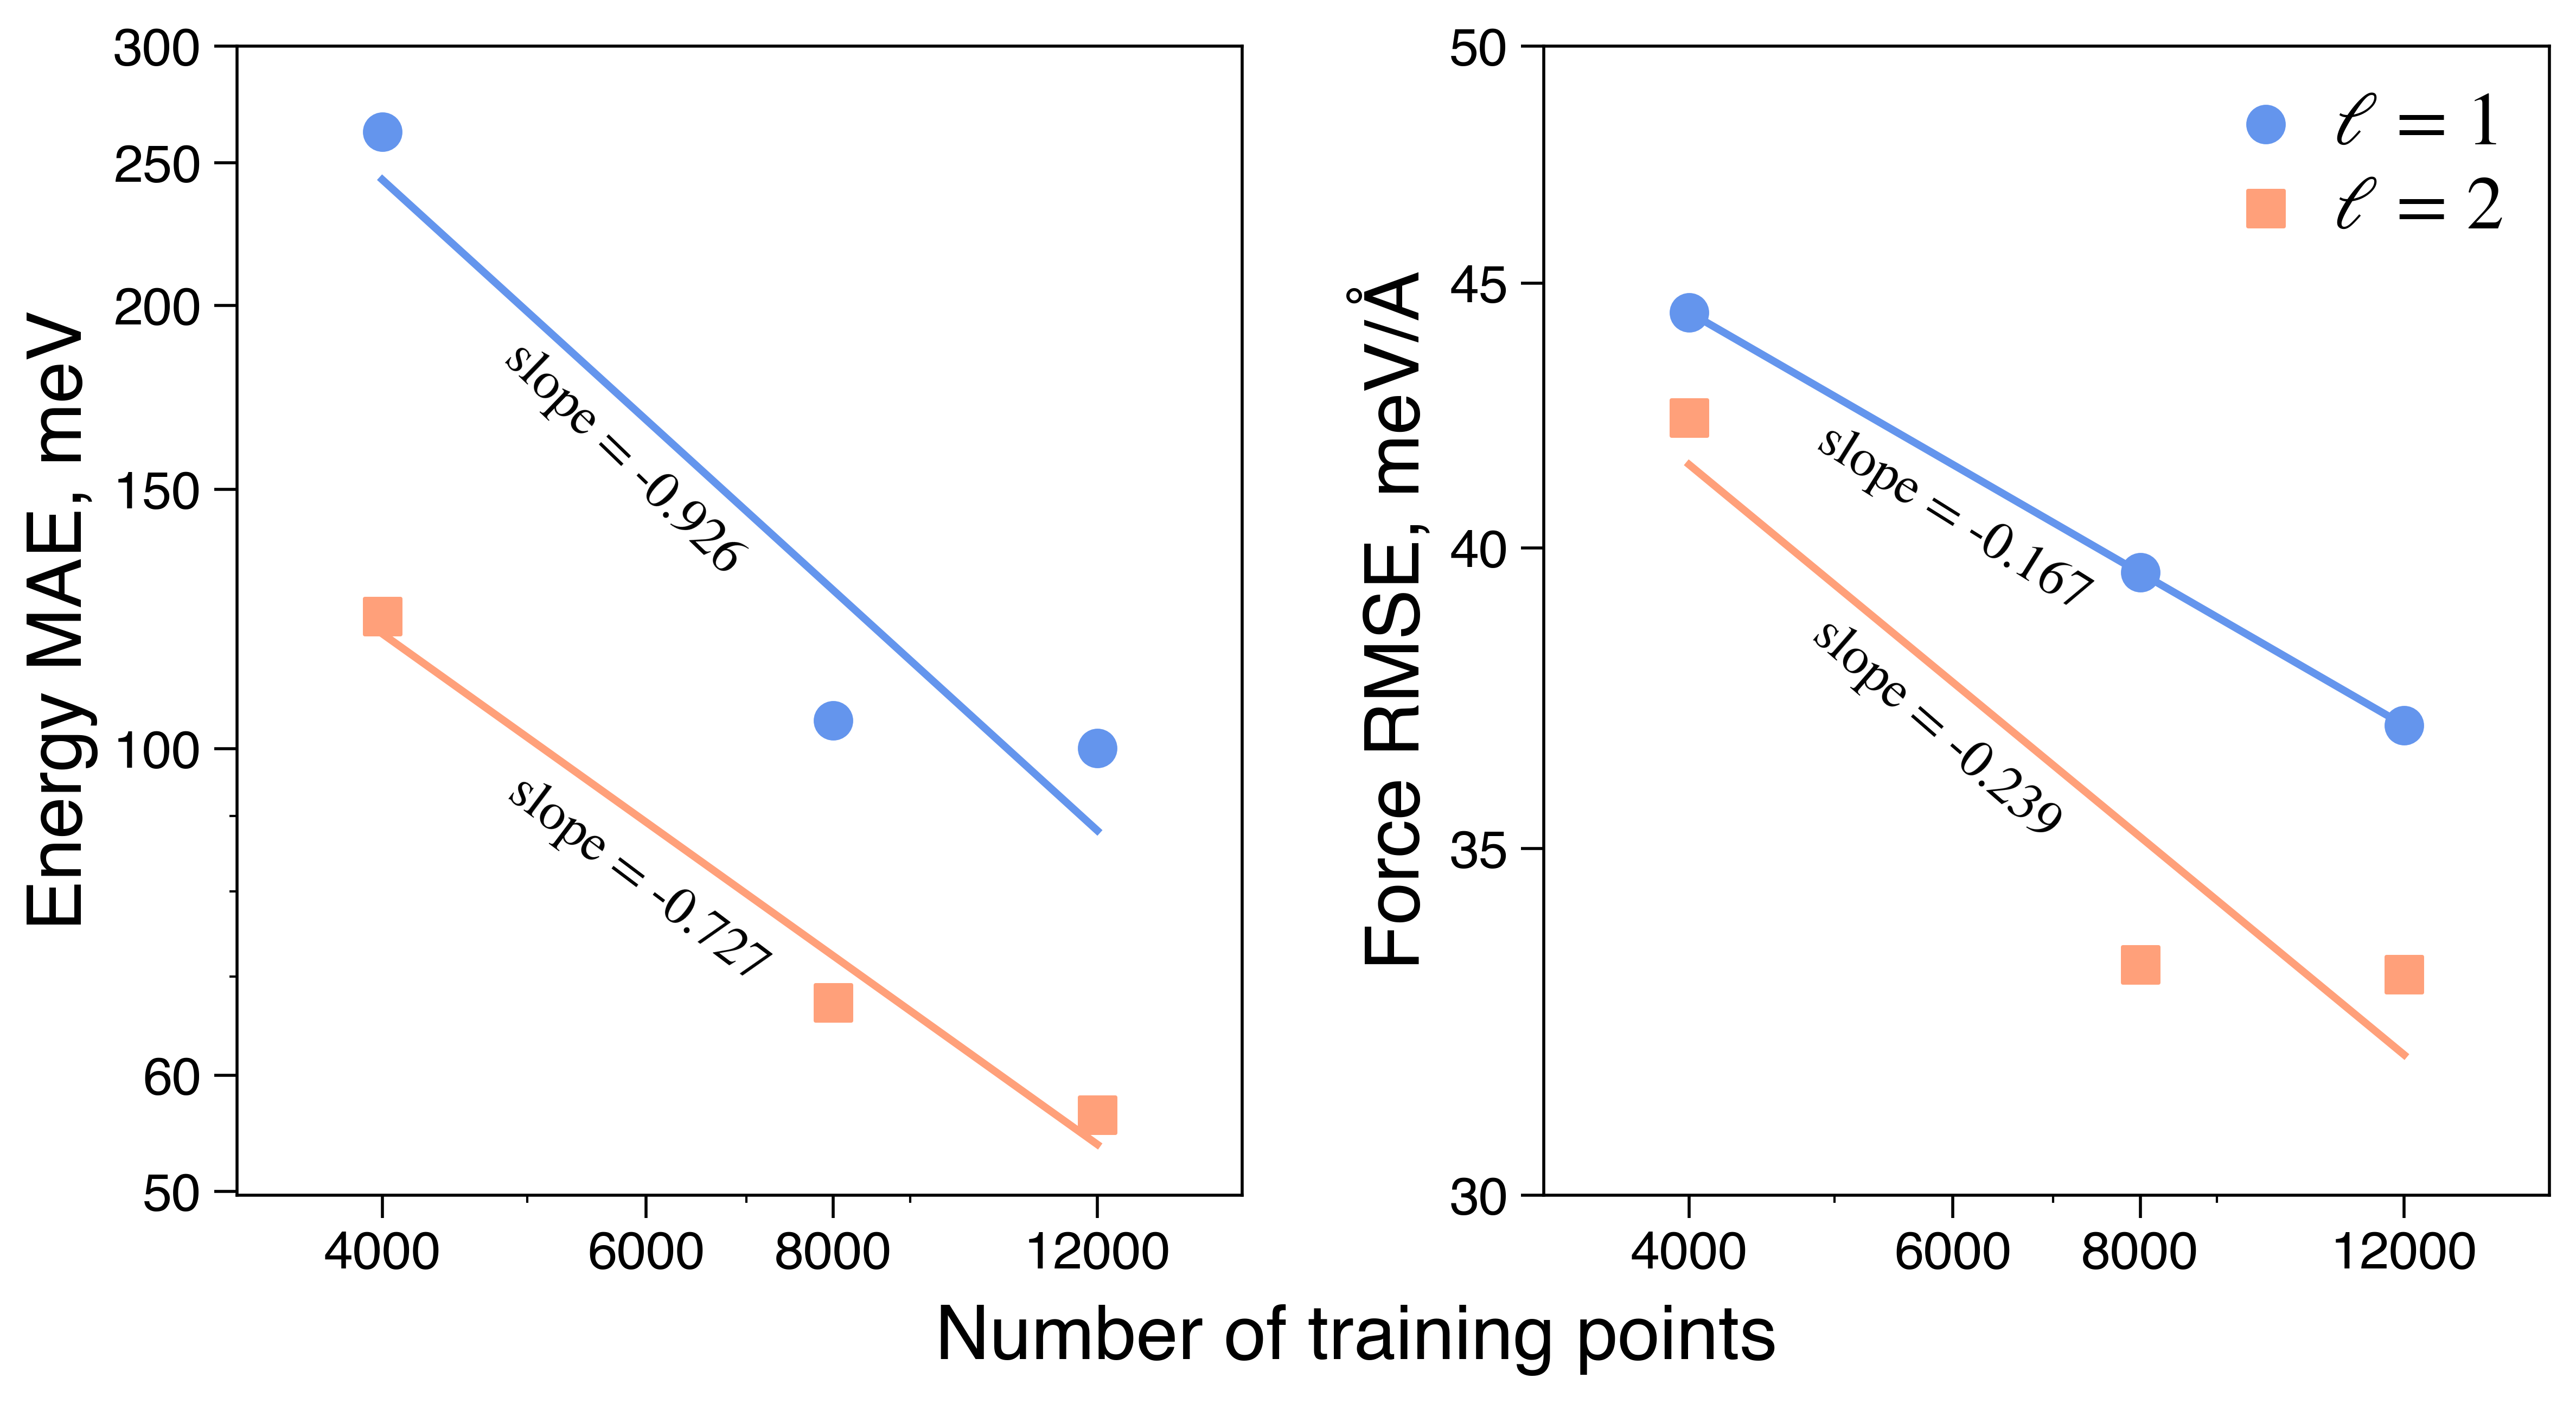
\includegraphics[width=0.8\textwidth]{Figures/4_Results/results_nnp_loglog_energy_force.png}
    \caption{Log-log plot of the errors in the energy and forces for the neural network potential with respect to the training dataset size. In all cases, the errors were calculated on the final test set of 1,800 data points.}
    \label{fig:nnp_log-log}
\end{figure}

The generalisability of the potentials can be further assessed by analysing how the errors in the energy and forces vary with the training dataset size. Figure~\ref{fig:nnp_log-log} shows a log-log plot of these errors for the \ac{nnp} at each iteration of the learning loop. The errors were evaluated \textit{a posteriori} on the final test set of 1,800 data points.

By examining the slopes, it becomes evident that the dataset size significantly influences how well the network learns the energies. The errors in the forces, however, are less sensitive to dataset size, which is reasonable given that the forces are not predicted directly by the network, but rather computed as the derivative of the energy with respect to atomic positions. Interestingly, the \acp{nnp} began producing sufficiently accurate results after the second training round, i.e., with 8,000 data points. This suggests that a dataset of 12,000 points is indeed sufficient to achieve a very good fit.

\begin{figure}[t]
    \centering
    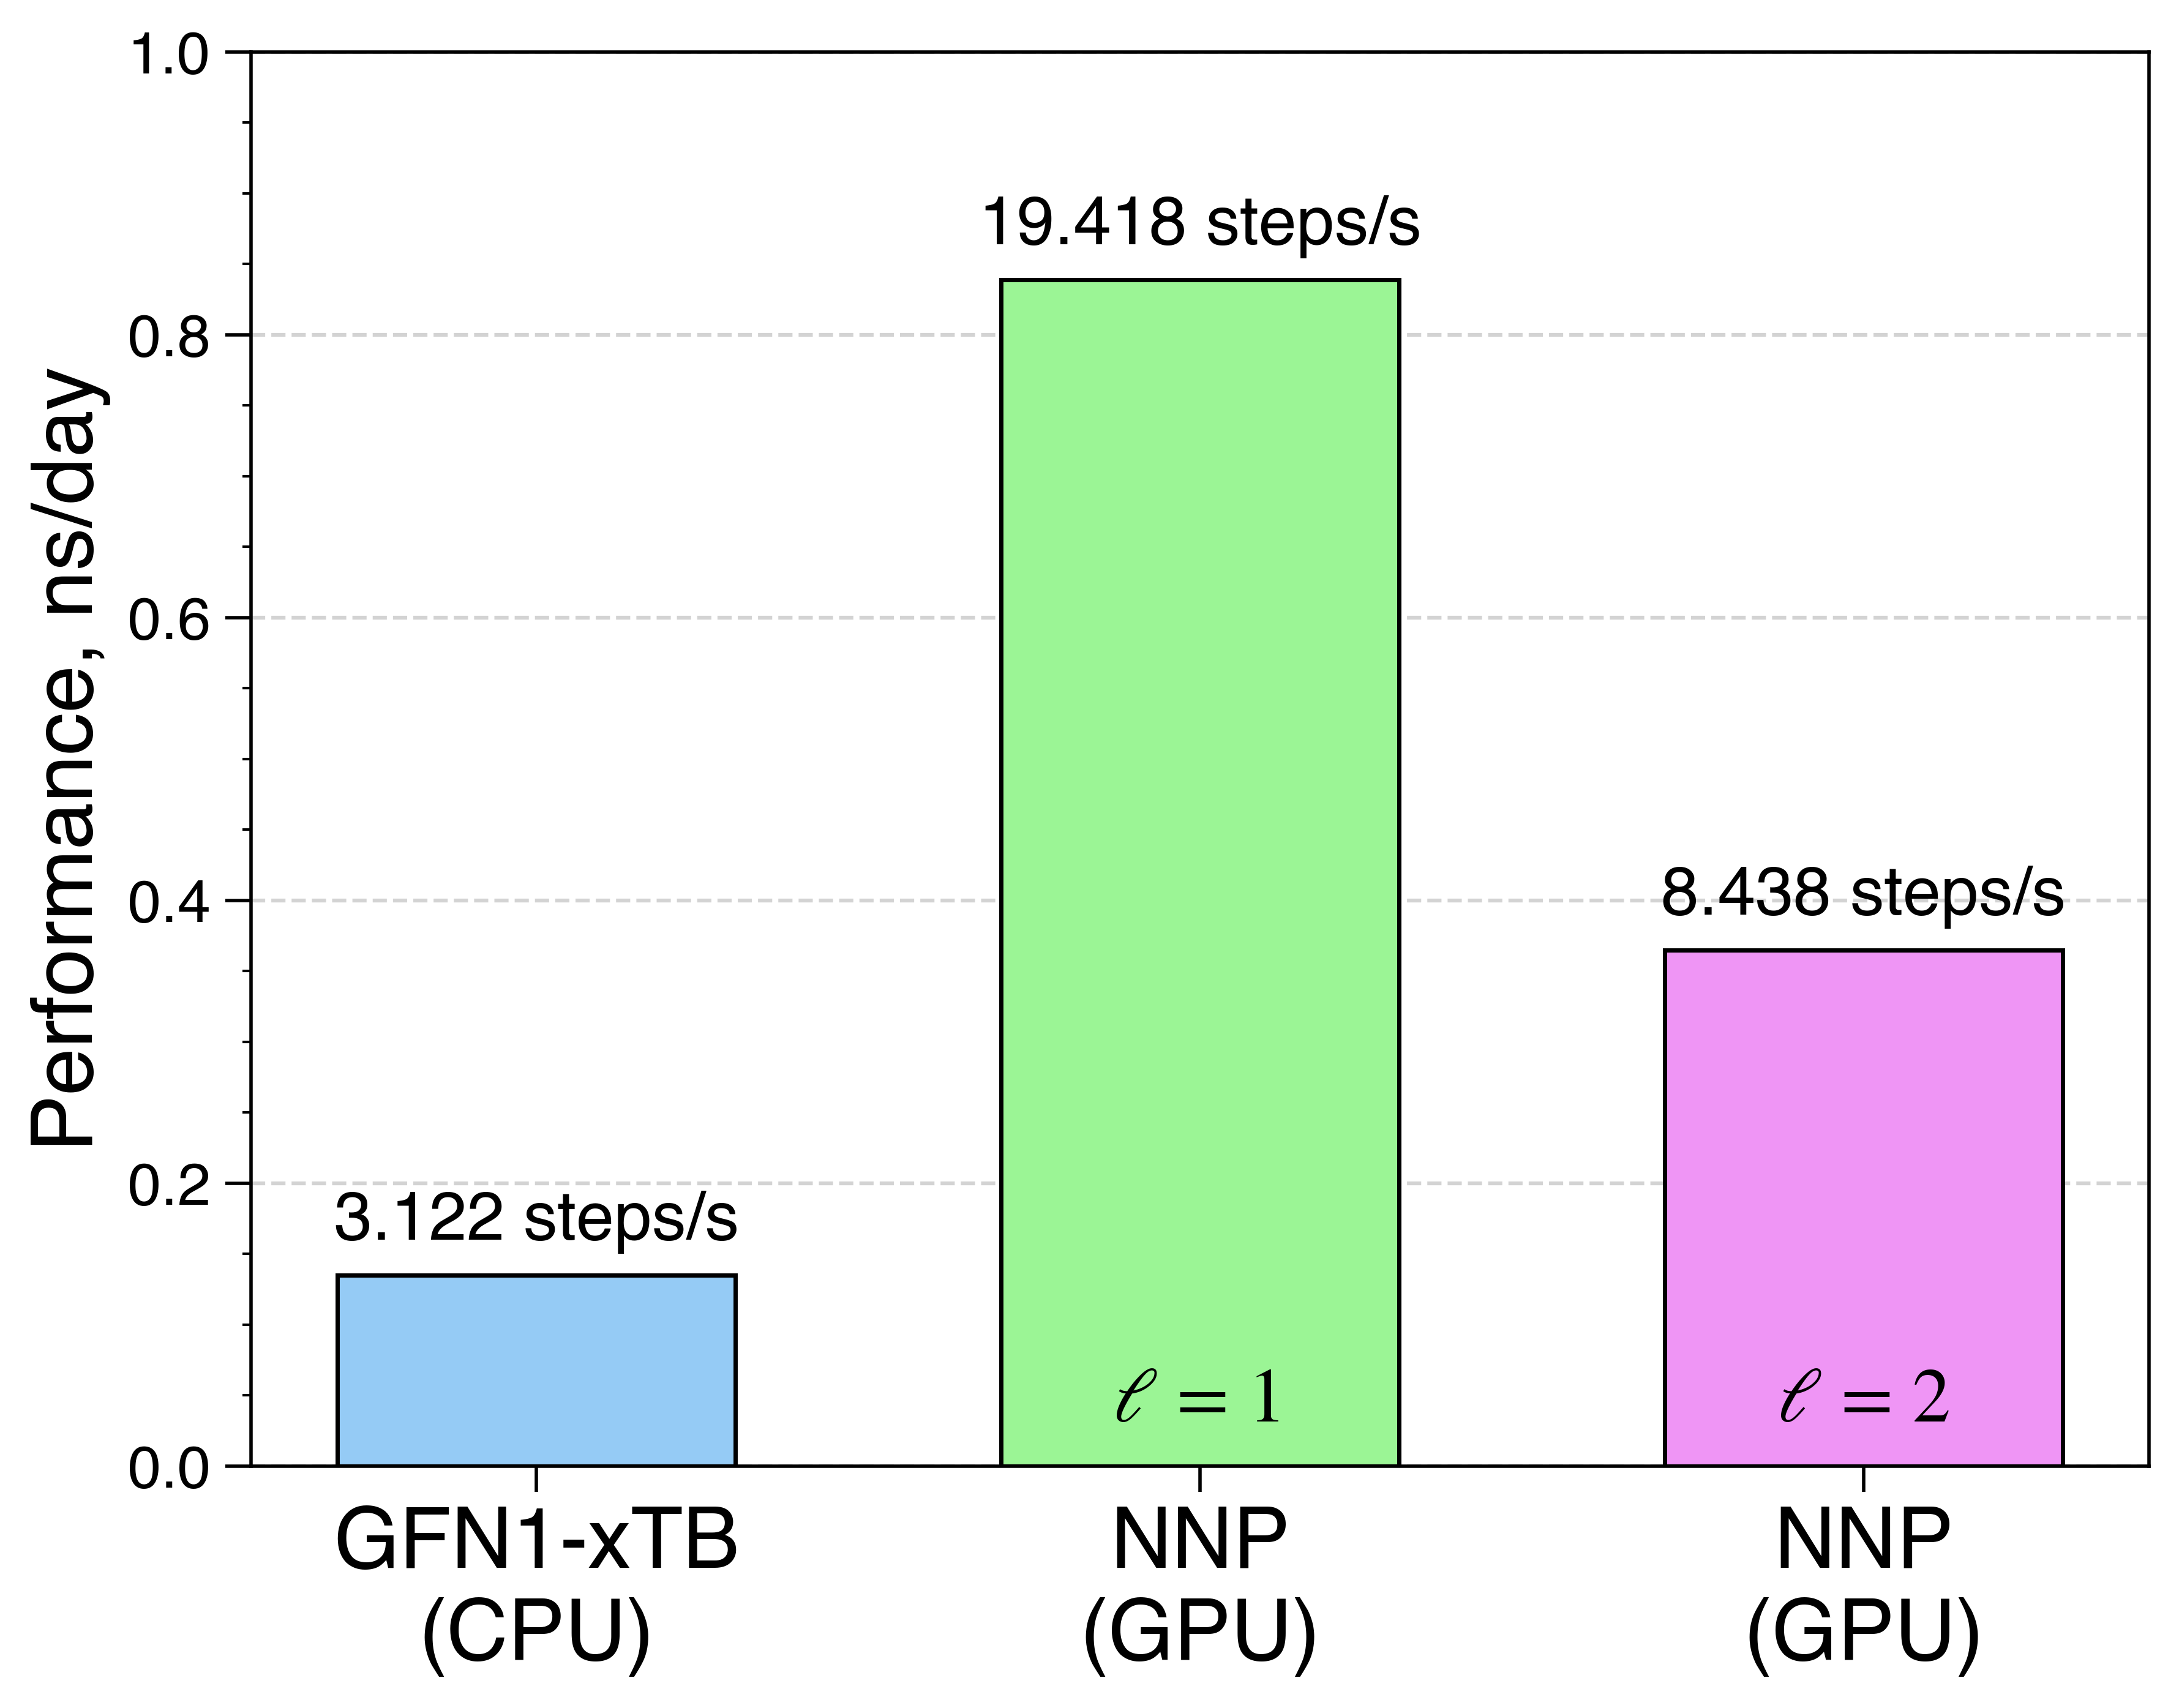
\includegraphics[width=0.6\textwidth]{Figures/4_Results/results_performance_comparison.png}
    \caption{Comparison of the performance between the \textit{ab initio} molecular dynamics runs driven by GFN1-xTB and neural network potentials fitted with different tensor ranks. CPU = 2 Intel Xeon Platinum 8468 CPUs (Sapphire Rapids), 48 cores each. GPU = 1 NVIDIA A100 80~GB GPU.}
    \label{fig:performance_comparison}
\end{figure}

The next question to address is which of the two \acp{nnp} should be used in subsequent calculations. To answer this, the performance of the potentials was compared in terms of computational time required to run \ac{aimd} simulations. The results are presented in Figure~\ref{fig:performance_comparison}. The \ac{aimd} simulations were performed on the \ac{medp} system.

It is clear that the \ac{nnp} with $\ell=1$ is significantly more efficient than both the $\ell=2$ \ac{nnp} and GFN1-xTB. It is important to highlight that the number of trainable parameters in the $\ell=1$ \ac{nnp} is 206,520, whereas for $\ell=2$ it is 452,280, making the latter nearly twice as slow in evaluating energies and gradients. Most likely, the performance of the \ac{pbe} functional would be considerably slower - so much so that its bar would not appear on the plot.

Taking both accuracy and performance into account, the \ac{nnp} with $\ell=1$ was selected for further calculations. It is sufficiently accurate to describe the reaction mechanism, and fast enough to allow for extended \ac{aimd} simulations. The \ac{nnp} with $\ell=2$ could be used in future work if an even more accurate potential is required.



%%%%%%%%%%%%%%%%%%%%%%%%%%%%%%%%%%%%%%%%%%%%%%%%%%%%%%%%%%%%%%%%%%%%%%%%%%%%%%%%
\section{Stability of the production runs}

\begin{figure}[b!]
    \centering
    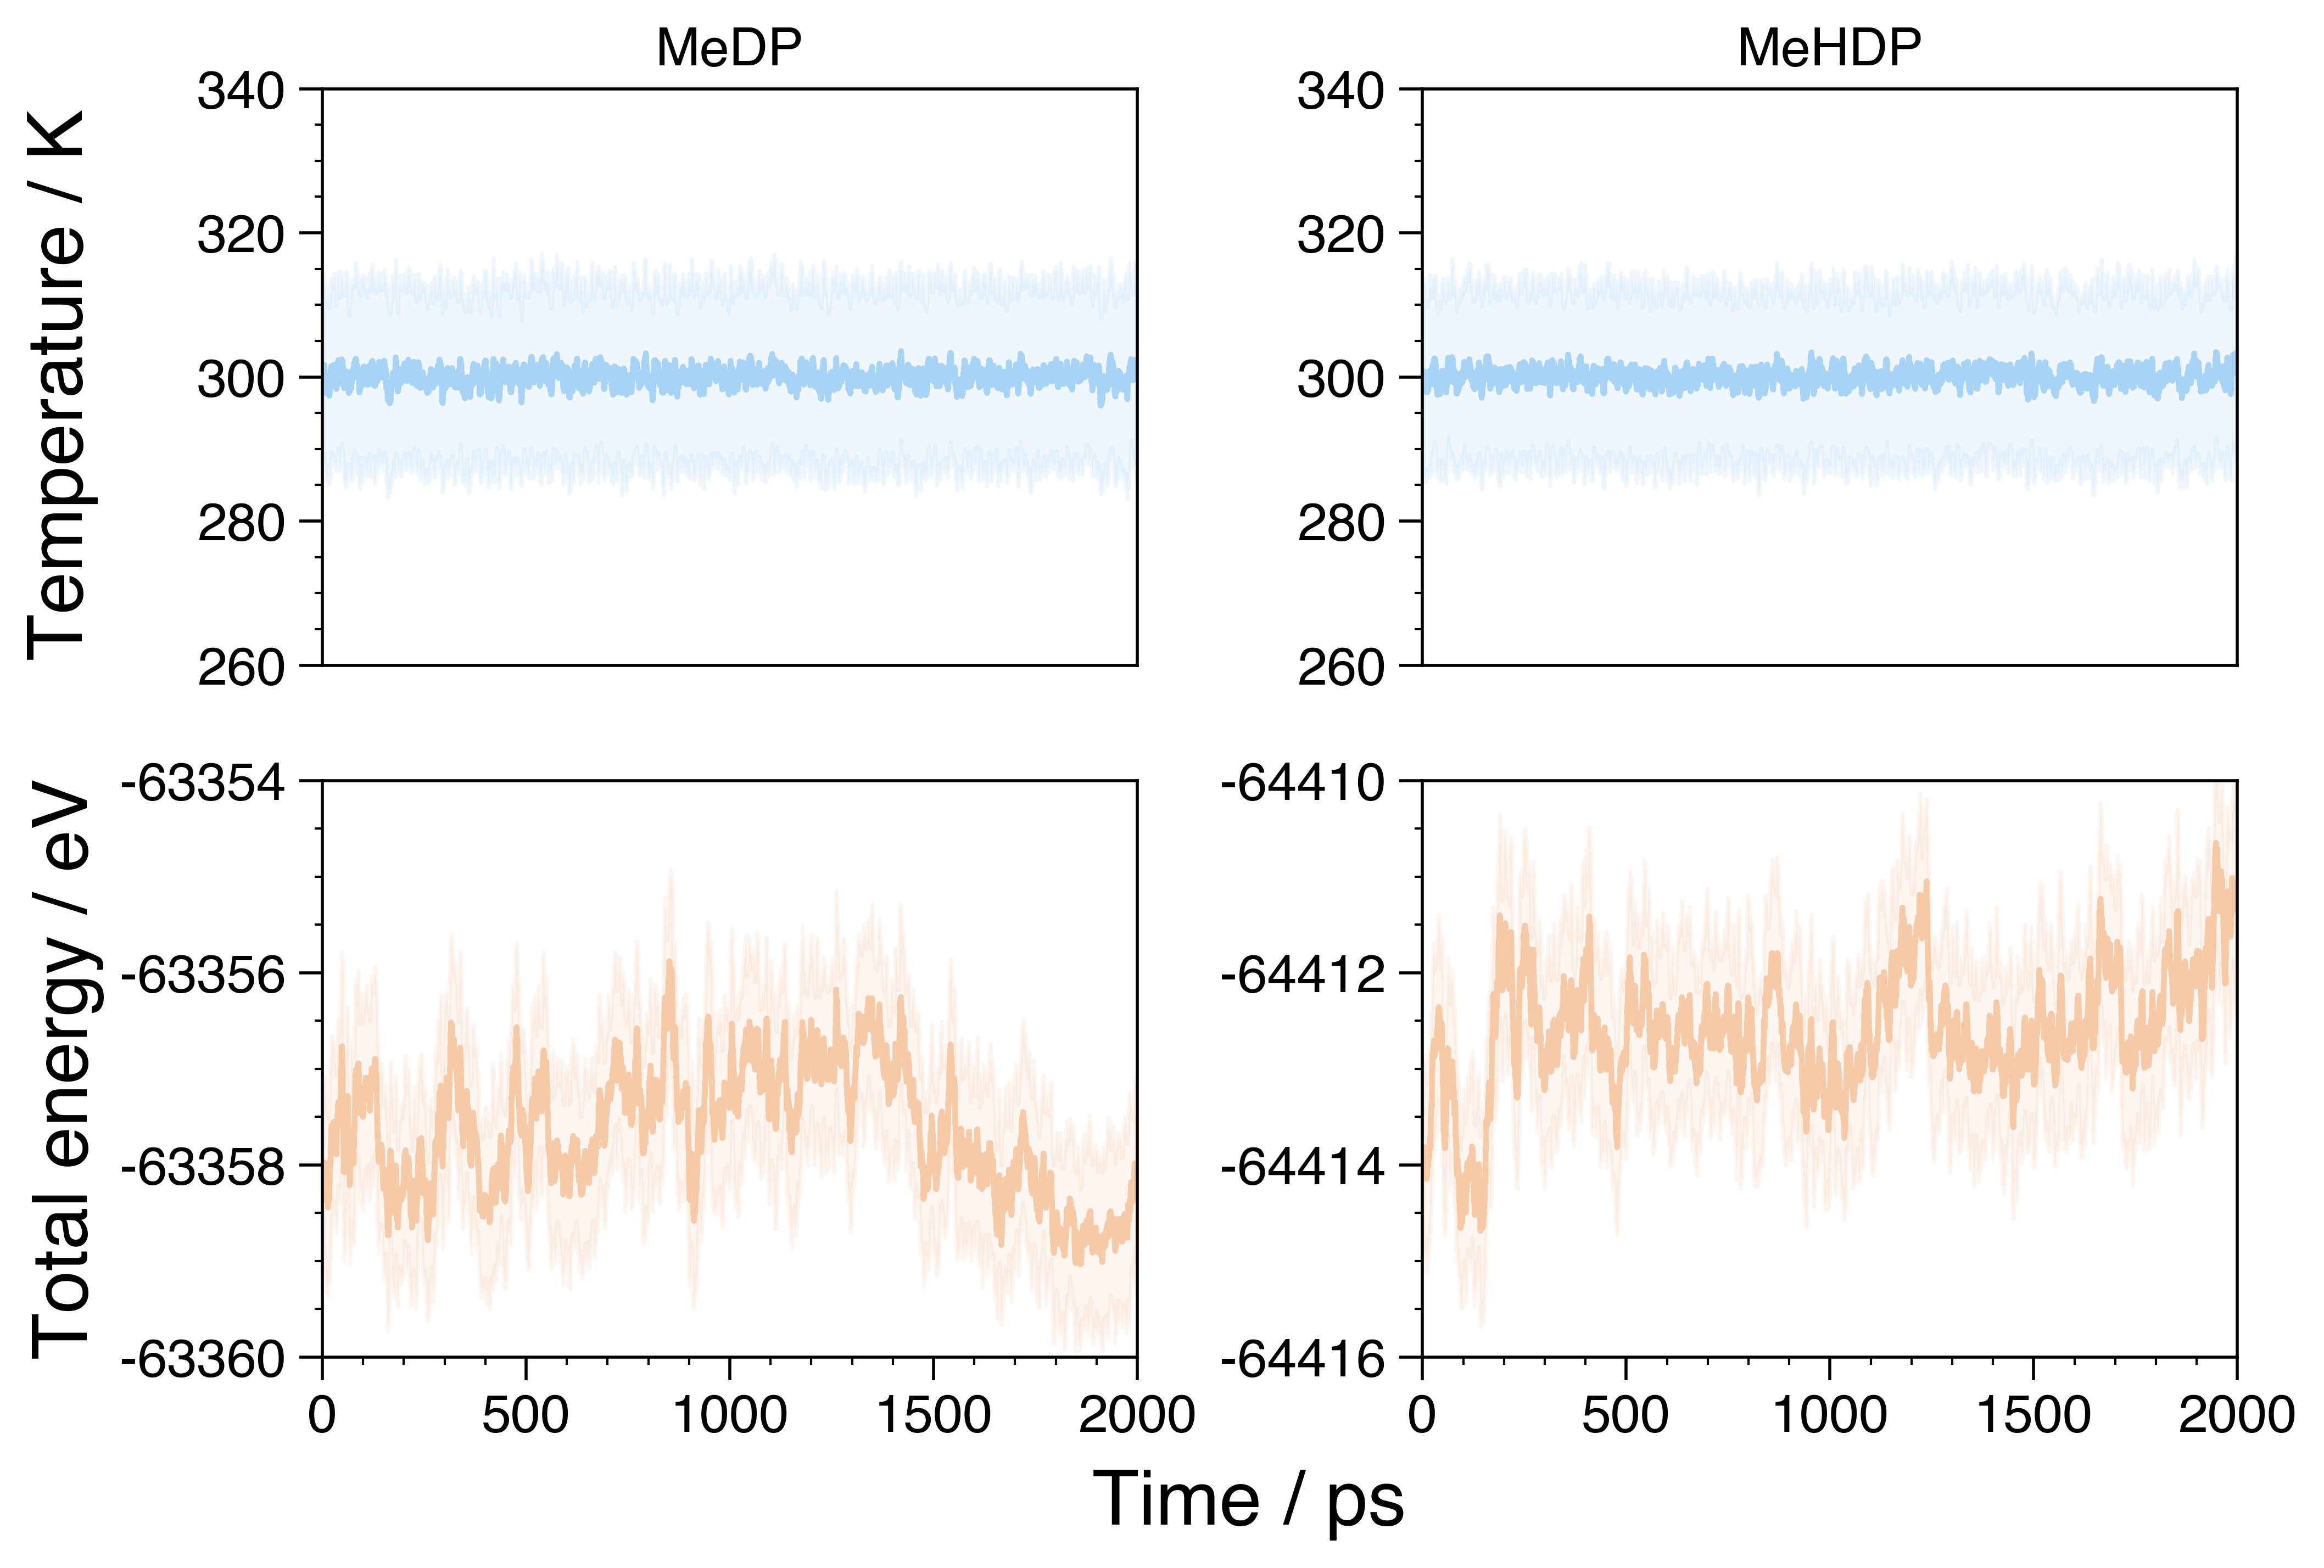
\includegraphics[width=0.8\textwidth]{Figures/4_Results/results_aimd_stability.png}
    \caption{Temperature and total energy fluctuations during the production runs at 300 K. The solid line represents the average, while the shaded area indicates the standard deviation. The average and the standard deviation were calculated using a sliding window of 1 ps.}
    \label{fig:temp_energy_fluctuations}
\end{figure}

Before discussing the reaction mechanism and the free energy profiles, it is important to assess the quality of the fitted \ac{nnp} in a real world scenario. To do so, we can briefly touch upon the stability of the production runs. The stability of the \ac{aimd} simulations was assessed by monitoring temperature and total energy fluctuations over time. The corresponding results are presented in Figure~\ref{fig:temp_energy_fluctuations}.

Temperature control was achieved using the Nos\'e--Hoover thermostat, while the total energy was calculated as the sum of potential and kinetic energies. The production runs were carried out at 300 K, and indeed, the average temperature remained close to this target, with a standard deviation of approximately 10 K. As expected for the \ac{nvt} ensemble, the total energy showed some fluctuations, yet remained within reasonable bounds in the simulations for both \ac{medp} and \ac{mehdp} systems.

It was of particular interest to evaluate the stability of the simulations driven by the \ac{nnp}. These simulations remained stable, exhibiting neither system explosions nor any other artefacts over the 4,000,000 time steps corresponding to 2 ns. This indicates the absence of extreme force values that could have caused numerical instabilities. In a recent study~\citep{fuForcesAreNot2023}, the authors compared the stability of \ac{aimd} simulations driven by equivariant and invariant \acp{nnp}, and found that NequIP was among the most stable potentials tested across various systems. The robustness of the fitted by NequIP \ac{nnp} employed in this work is consistent with those findings.



%%%%%%%%%%%%%%%%%%%%%%%%%%%%%%%%%%%%%%%%%%%%%%%%%%%%%%%%%%%%%%%%%%%%%%%%%%%%%%%%
\section{Radial distribution function of water} \label{sec:water_rdf}

\begin{figure}[b!]
    \centering
    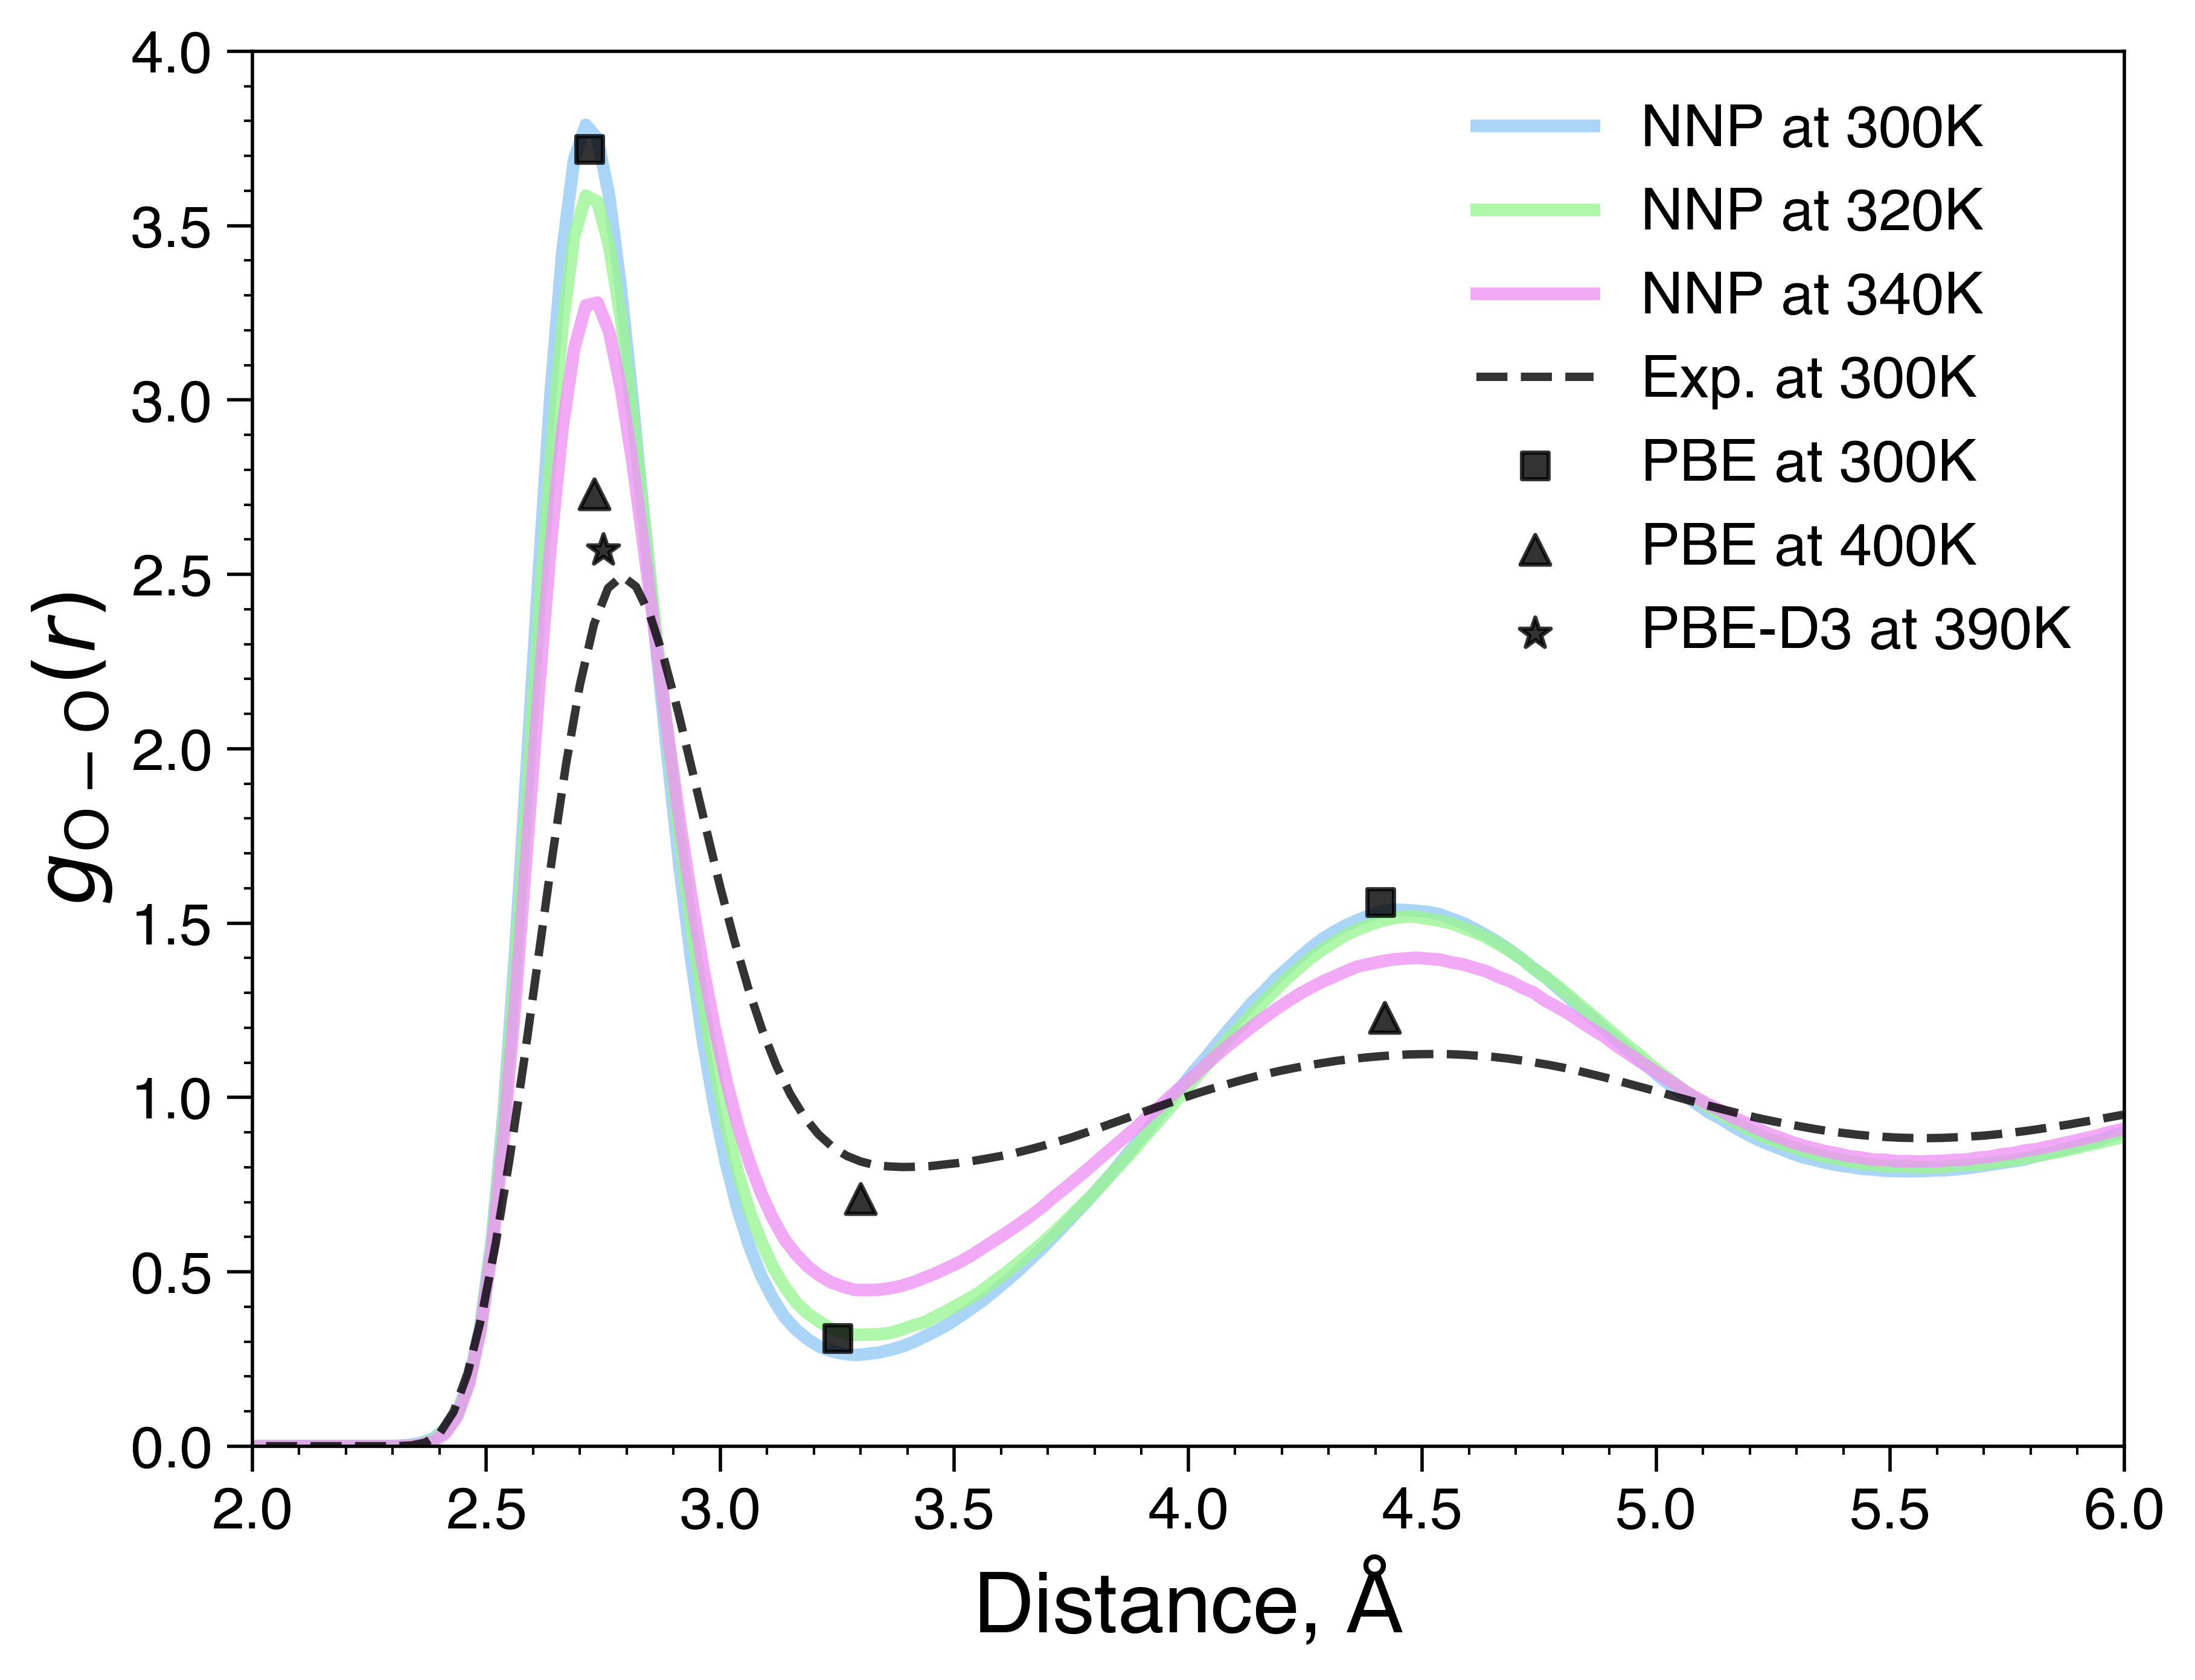
\includegraphics[width=0.6\textwidth]{Figures/4_Results/results_water_rdf.png}
    \caption{Oxygen-oxygen \ac{rdf} of water calculated from a production run at 300 K. Experimental data was taken from~\citep{soperRadialDistributionFunctions2013}. The PBE and PBE-D3 data were taken from \citep{phamStructureDynamicsAqueous2016} and \citep{zhouQuantifyingStructureWater2022}, respectively.}
    \label{fig:water_rdf}
\end{figure}

The quality of the \ac{nnp} can be further assessed by comparing the \ac{rdf} of water calculated from the production runs with experimental data and previously reported computational findings. The oxygen-oxygen RDF obtained from the \ac{medp} production run is shown in Figure~\ref{fig:water_rdf}.

It is evident that the \ac{nnp} is in qualitative agreement with the experimental data. However, it overestimates the heights of the first two peaks and underestimates the depth of the first minimum. For the \ac{nnp}, the first maximum occurs at 2.7188~\AA\ with a height of 3.8189, while the first minimum is located at 3.2813~\AA\ with a value of 0.2515. The second maximum appears at 4.4938~\AA\ with a height of 1.5725. There is also a slight shift to the left in the position of the peaks in comparison to the experimental data.

One could argue that the accuracy of the fitted \ac{nnp} is inherently limited by the quality of the training data. In this study, the dataset was labelled at the PBE-D3(BJ)/TZV2P level of theory. Accordingly, the resulting oxygen-oxygen water \ac{rdf} is consistent with the \ac{aimd} study where the \ac{rdf} was calculated using the \ac{pbe} functional~\citep{phamStructureDynamicsAqueous2016} as can be found in Figure~\ref{fig:water_rdf}.

It has previously been shown that, in order to obtain a more accurate representation of the bulk water structure, the system temperature should be increased. For instance, \citep{zhouQuantifyingStructureWater2022} reported that the PBE functional with the Grimme's D3 dispersion correction yields a more accurate \ac{rdf} at 390 K. A similar trend was observed for the \ac{pbe} functional~\citep{phamStructureDynamicsAqueous2016}, with better agreement with experimental data achieved at 400 K.

In this work, the production runs were conducted at 300 K. Thus, the resulting structure and dynamics of water will be less accurately captured than at elevated temperatures. Nevertheless, it remains in good agreement with what would be expected from the \ac{pbe} functional.



%%%%%%%%%%%%%%%%%%%%%%%%%%%%%%%%%%%%%%%%%%%%%%%%%%%%%%%%%%%%%%%%%%%%%%%%%%%%%%%%
\section{Convergence of the free energy profiles}

\begin{figure}[t!]
    \centering
    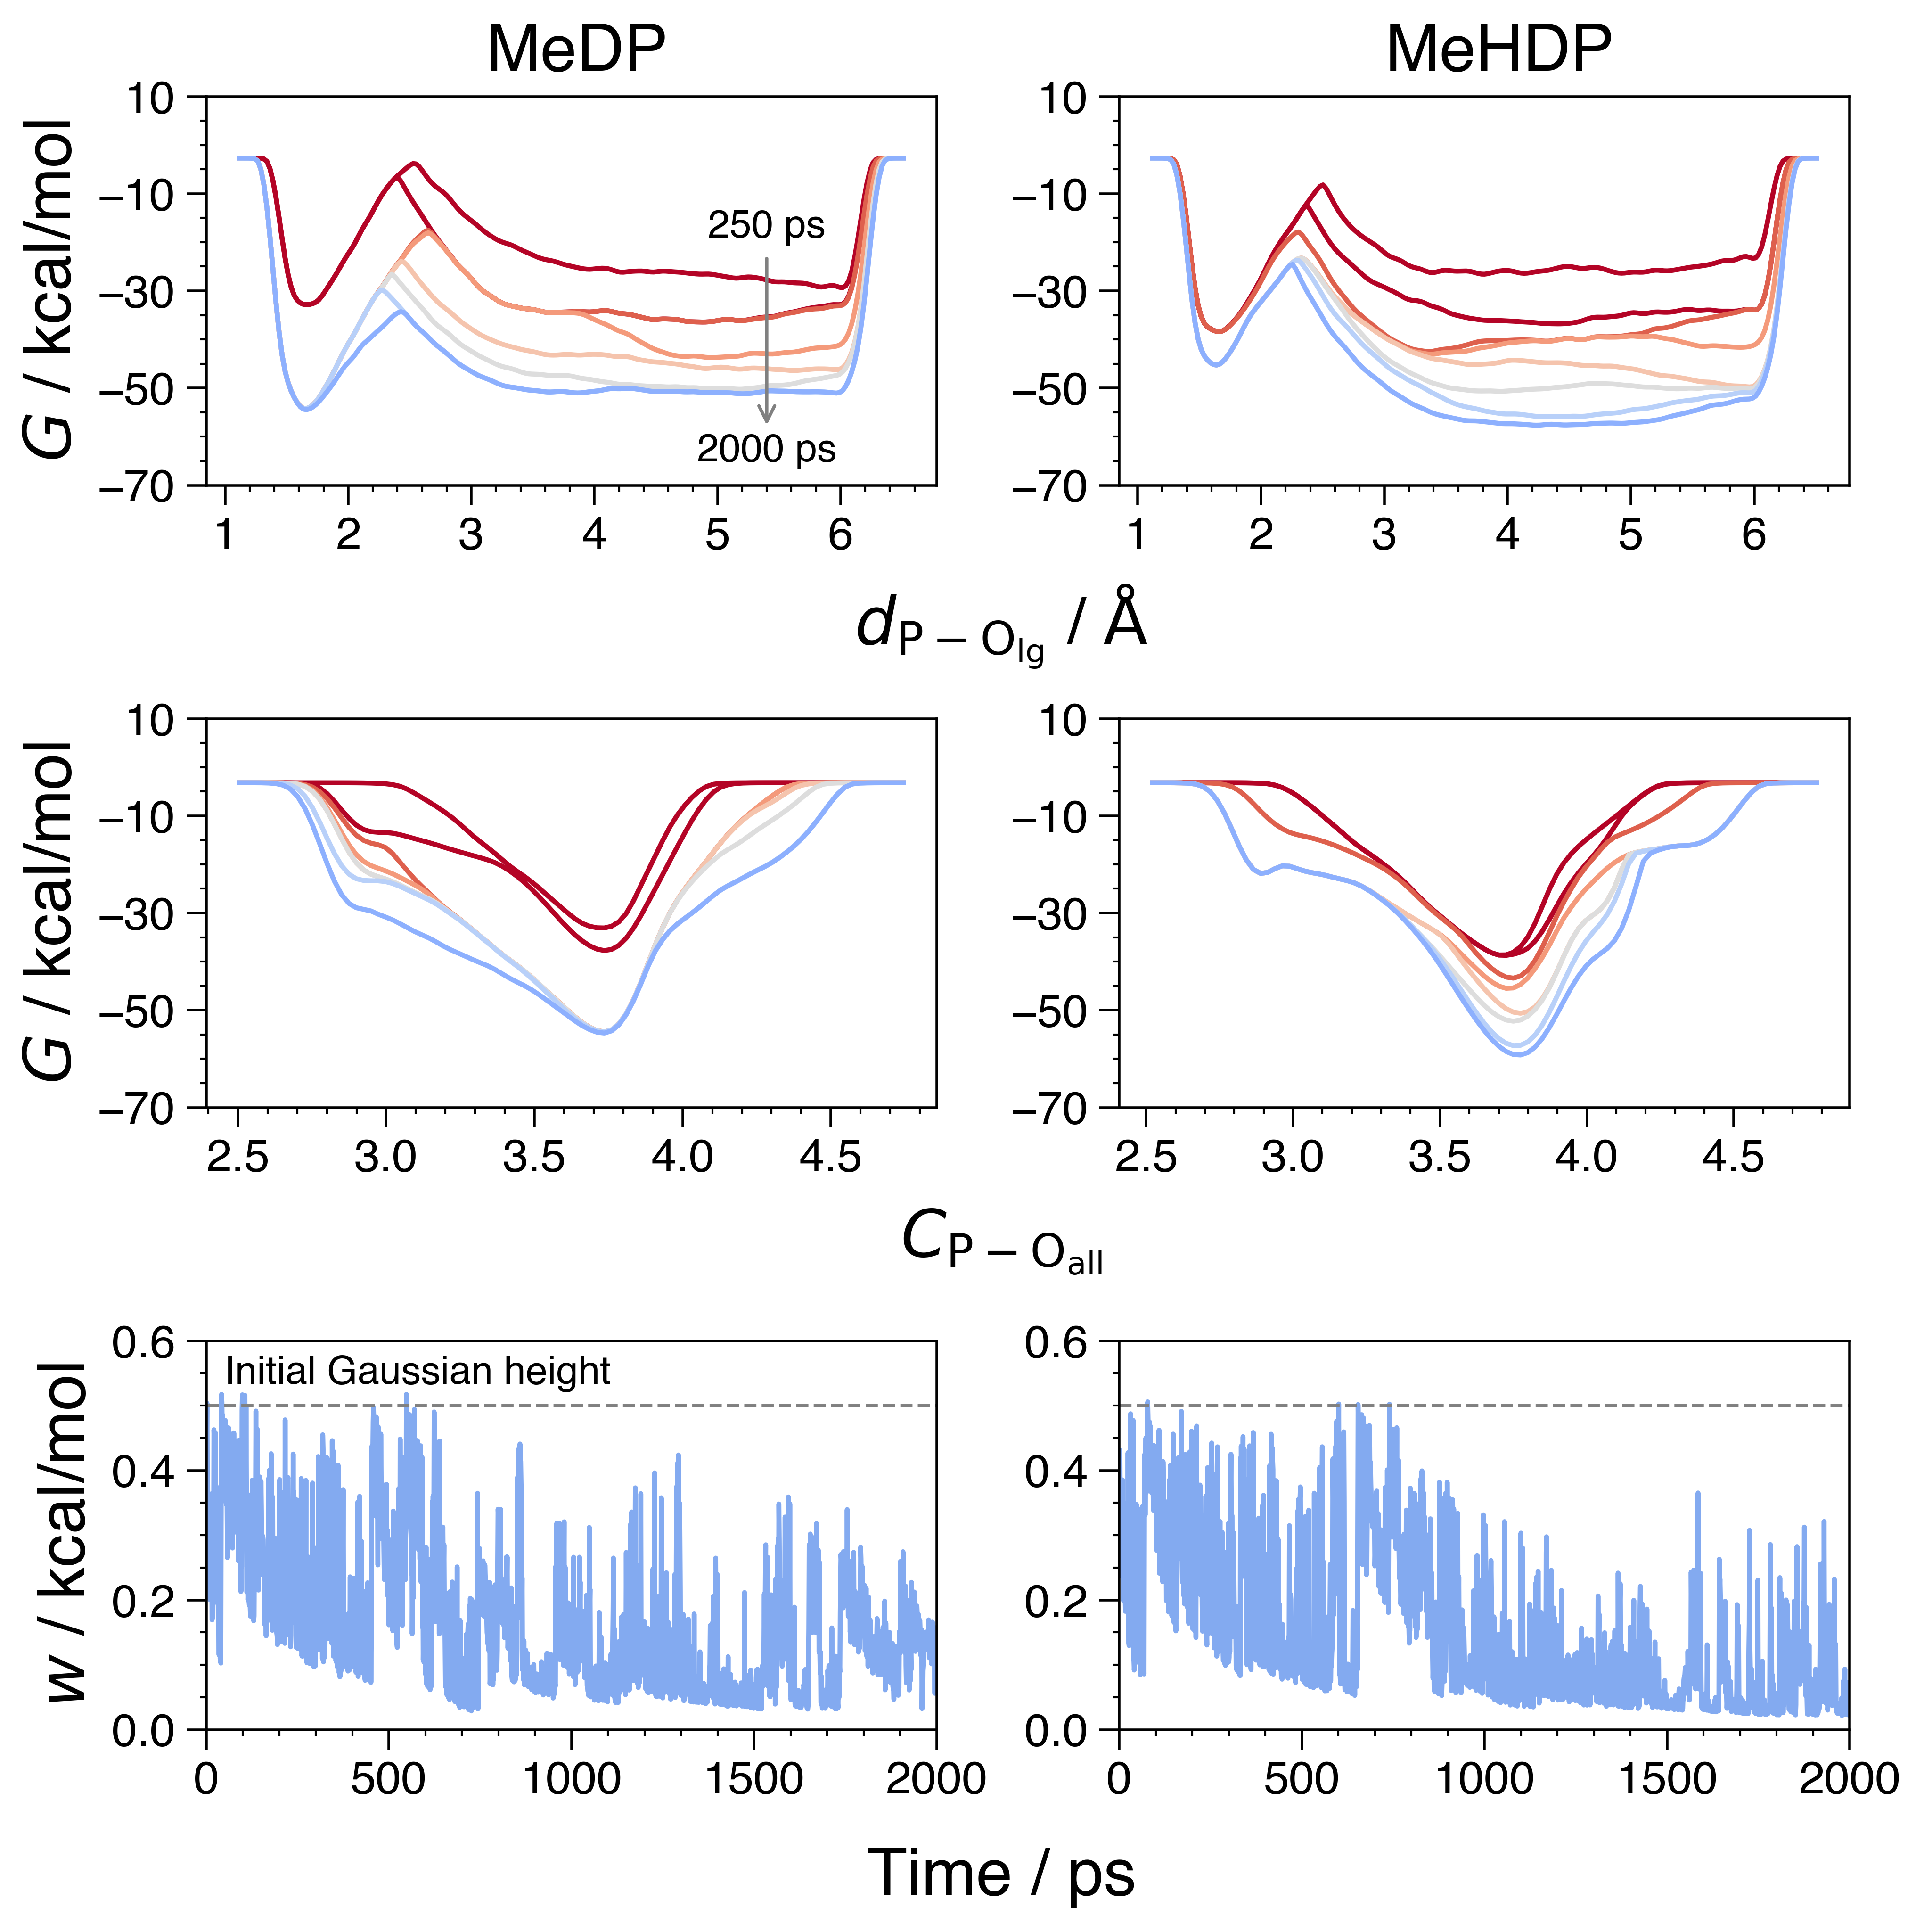
\includegraphics[width=0.85\textwidth]{Figures/4_Results/results_300K_fes_convergence.png}
    \caption{\ac{fes} convergence and the evolution of the applied Gaussian biasing potential during the production runs of \ac{medp} (left panel) and \ac{mehdp} (right panel). Free energy surfaces were projected on one \ac{cv}, namely the distance (first row) and the coordination number (second row). They were calculated every 250 ps. The third row shows the evolution of the Gaussian biasing potential with the initial height of 0.5 kcal/mol.}
    \label{fig:300k_fes_convergence}
\end{figure}

A vital aspect of any enhanced sampling-based study is the convergence of the \ac{fes}. In this work, convergence was monitored by examining the evolution of the free energy profiles and the height of the applied Gaussian kernels over time. The results for the production runs are presented in Figure~\ref{fig:300k_fes_convergence}.

The left panel shows the convergence of the \ac{fes} for the \ac{medp} system, while the right panel shows the corresponding results for the \ac{mehdp} system. Gaussian kernels were deposited every 100 \ac{md} steps, i.e., every 50 fs. Over the course of the 2 ns simulations, a total of 40,000 Gaussian kernels were added.

To evaluate the convergence of the \ac{fes}, the free energy profiles were calculated every 250 ps, i.e., after every 5,000 Gaussian kernels. One can clearly observe how the free energy profiles evolve over time. Initially, the \ac{fes} appears flatter and lies in higher energy regions. As the simulation progresses, the system explores a broader range of the \ac{fes}, including the reactant and product basins, as well as the \ac{ts}, and the free energy profile becomes more structured.

By examining the 1D free energy profiles in Figure~\ref{fig:300k_fes_convergence}, it is clear that they are not fully converged even after 2 ns of simulation time. The \ac{fes} continues to evolve in the \ac{ts} regions ($C_\mathrm{P-O_{\mathrm{all}}}<3.5 \; \mathrm{and} >3.9$) and the product basin ($d_\mathrm{P-O_{\mathrm{lg}}}>4.0$ \AA). The reactant state, on the other hand, appears to be well sampled, as it did not change during the final 250 ps of the simulation.

A similar trend can be observed in the evolution of the Gaussian biasing potential. Initially, the height of the Gaussian kernels is around 0.5 kcal/mol, as specified. As the simulation progresses, the Gaussian height gradually decreases. Occasional spikes in the height indicate that the system entered previously unexplored regions. In other words, when the system visits a new region of the \ac{fes}, the Gaussian height increases to ensure continued sampling in that region - an inherent feature of \ac{wtmd}.

It is not surprising that 2 ns of simulation time is insufficient, given the complexity of the \ac{fes}, even when projected onto just two \acp{cv}. It is also worth noting that, despite the relatively high rate of bias deposition, the applied bias itself is small. These factors contribute to slow convergence over long timescales, leading to a smoother \ac{fes}. For reference, in other studies involving \ac{nnp}-driven reactive events - such as urea decomposition~\citep{yangUsingMetadynamicsBuild2022}, phosphoester bond formation between orthophosphate and methanol~\citep{benayadPrebioticChemicalReactivity2024}, and glycine tautomerisation~\citep{zhangIntramolecularWaterMediated2024} - convergence was only reached after at least 6, 10, and 30 ns, respectively.

Although the free energy profiles obtained in this work are not fully converged, they show clear signs of progressing towards convergence. They are therefore expected to provide useful insights into the reaction pathways. It is important to keep this in mind when interpreting the results related to the reaction mechanism, particularly the kinetics and thermodynamics discussed in the following sections.



%%%%%%%%%%%%%%%%%%%%%%%%%%%%%%%%%%%%%%%%%%%%%%%%%%%%%%%%%%%%%%%%%%%%%%%%%%%%%%%%
\section{Evolution of the collective variables over time}

\begin{figure}[b!]
    \centering
    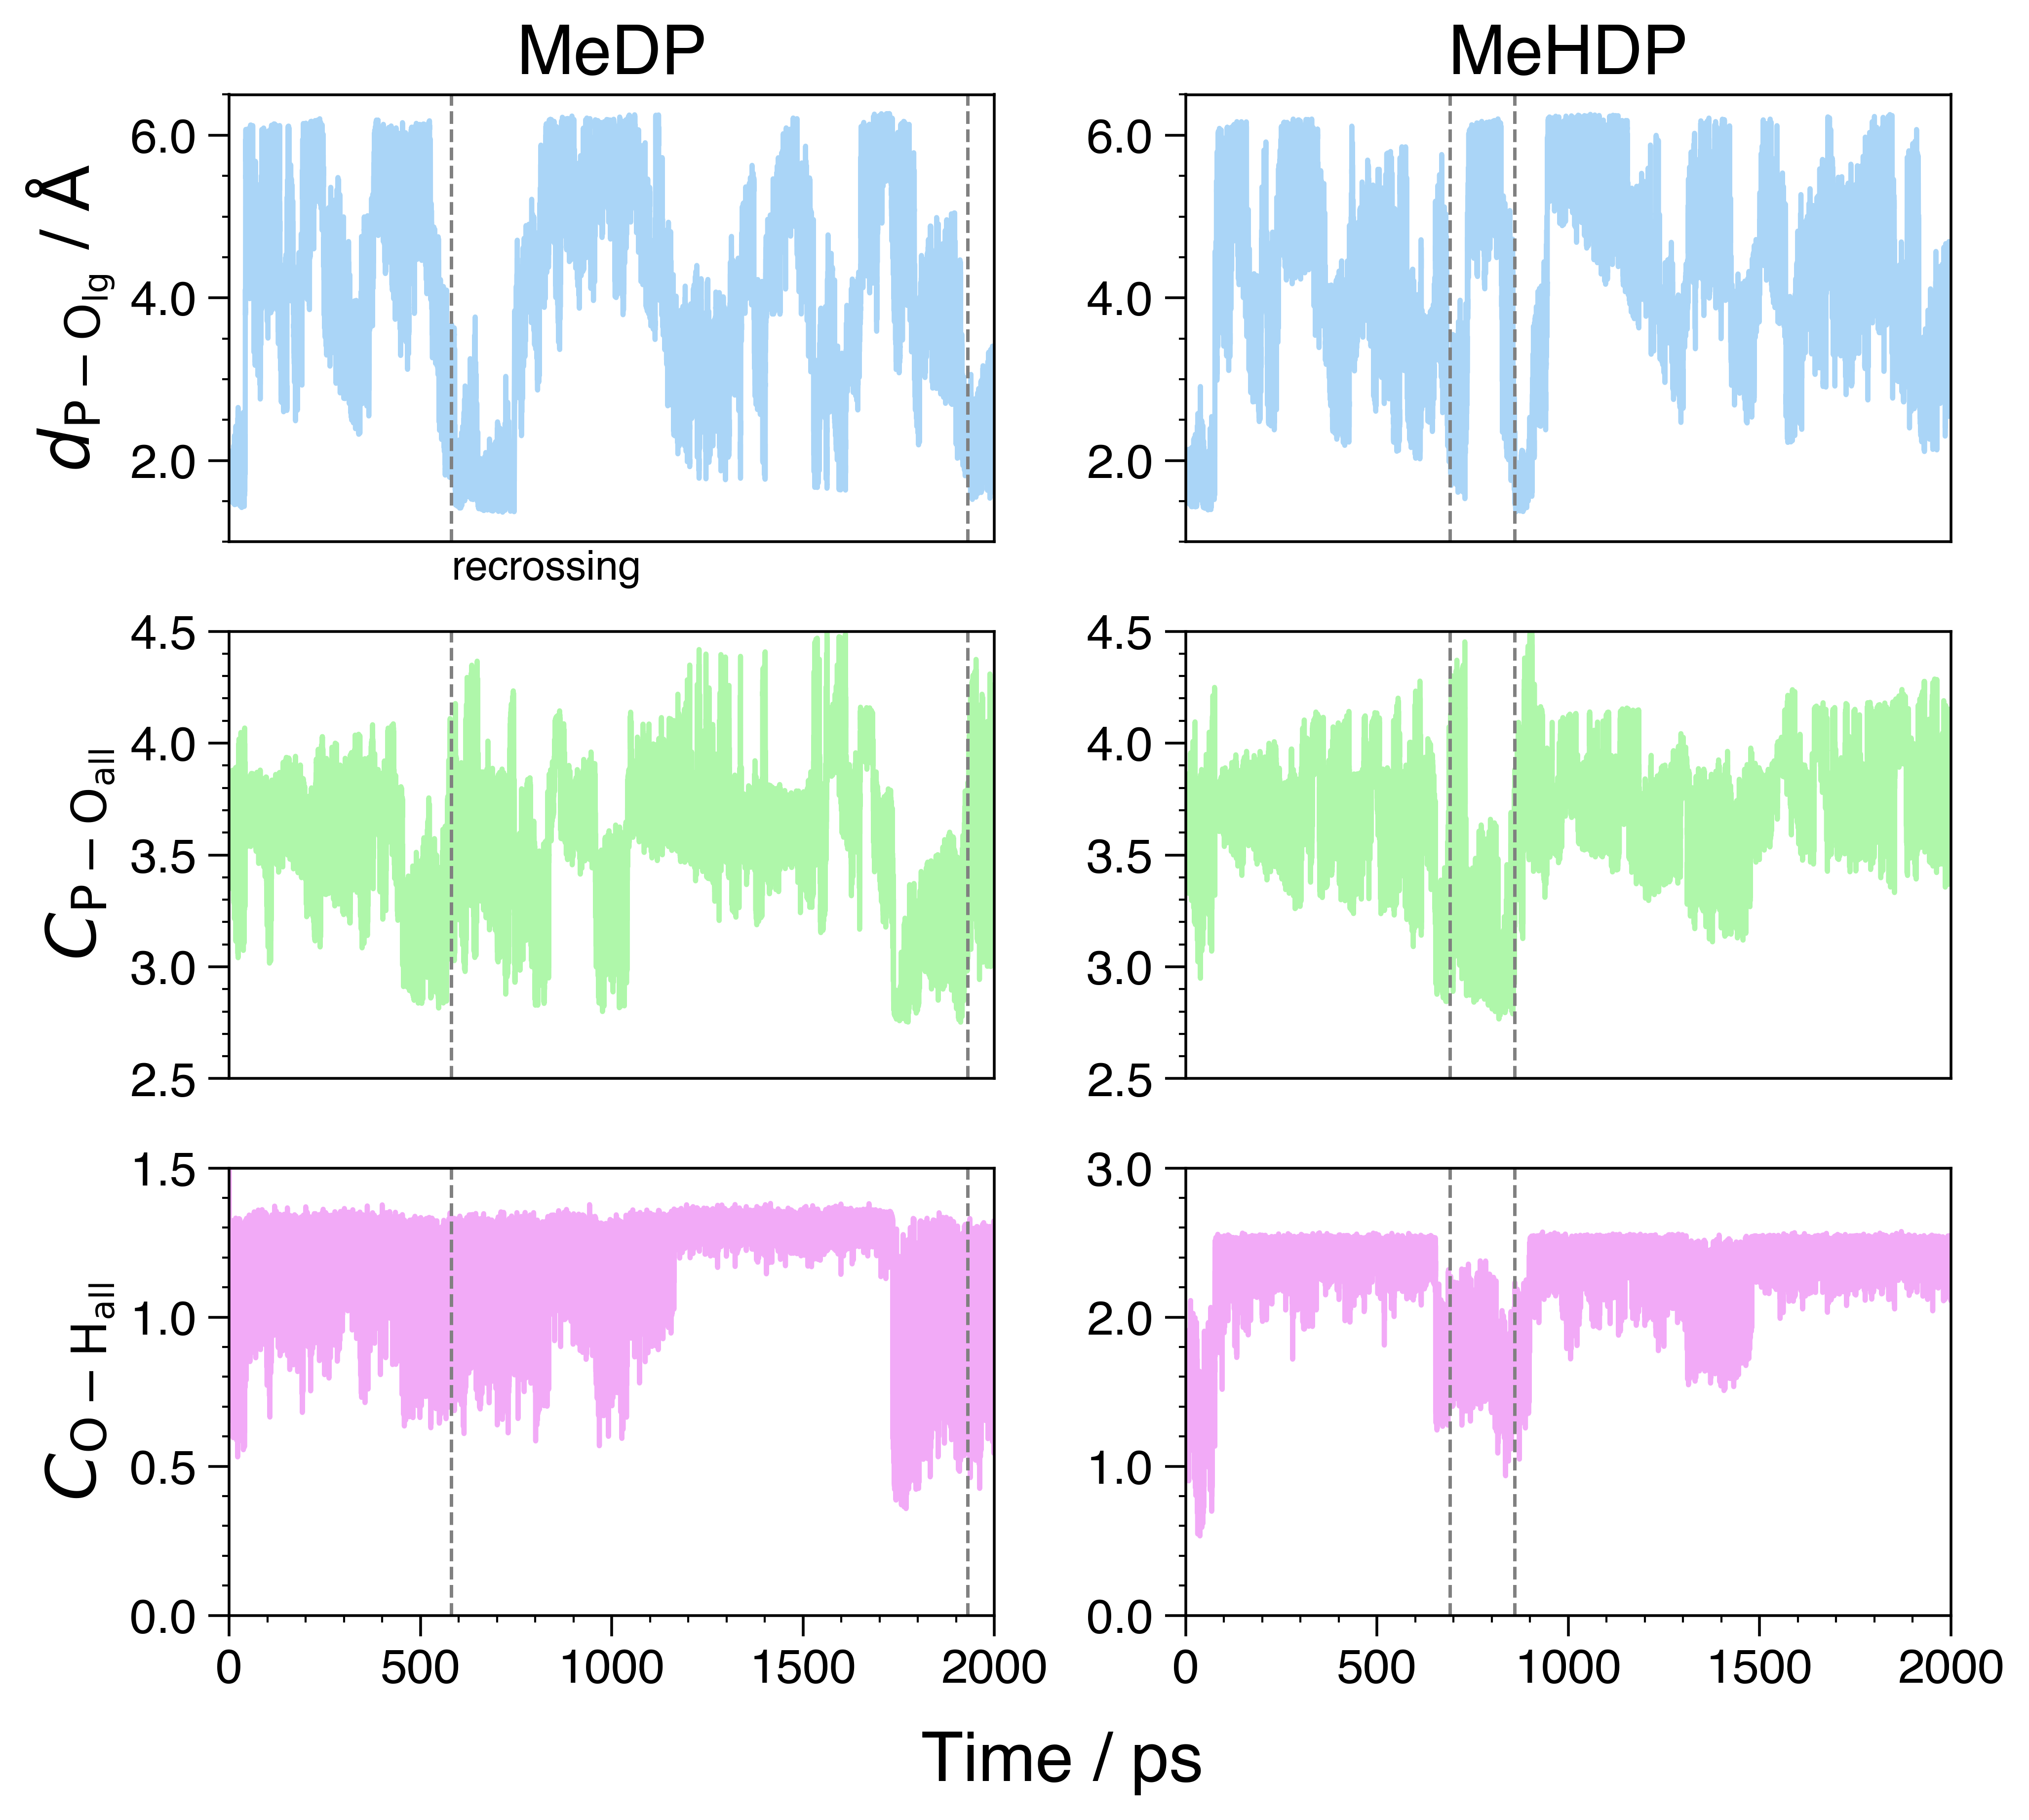
\includegraphics[width=0.85\textwidth]{Figures/4_Results/results_300K_cv_evolution.png}
    \caption{Evolution of the \acp{cv} during the production runs of \ac{medp} (left panel) and \ac{mehdp} (right panel). The first row shows the evolution of $d_\mathrm{P-O_{\mathrm{lg}}}$, the second row shows the evolution of $C_\mathrm{P-O_{\mathrm{all}}}$, and the third row shows $C_\mathrm{O-H_{\mathrm{all}}}$. The first two \acp{cv} were biased. Recrossings are indicated by the dashed lines.}
    \label{fig:300k_cv_evolution}
\end{figure}

Another way to assess the convergence and quality of the \ac{fes} is to examine how the \acp{cv} evolve over time, as shown in Figure~\ref{fig:300k_cv_evolution}.

The left panel presents the evolution of the \acp{cv} for the \ac{medp} system, while the right panel displays the corresponding results for the \ac{mehdp} system. The \acp{cv} depicted are: $d_\mathrm{P-O_{\mathrm{lg}}}$, $C_\mathrm{P-O_{\mathrm{all}}}$, and $C_\mathrm{O-H_{\mathrm{all}}}$. The first two \acp{cv} were biased during the \ac{wtmd} production runs, whereas the third was monitored to track the protonation state.

Let us first relate the \acp{cv} to the respective reaction states. In the reactant state, $d_\mathrm{P-O_{\mathrm{lg}}}$ is approximately 1.75~\AA, $C_\mathrm{P-O_{\mathrm{all}}}$ is around 3.75, and $C_\mathrm{O-H_{\mathrm{all}}}$ is less than 1.0/2.0 (\ac{medp}/\ac{mehdp}). In the product state, $d_\mathrm{P-O_{\mathrm{lg}}}$ exceeds 4.0~\AA, $C_\mathrm{P-O_{\mathrm{all}}}$ remains around 3.75, and $C_\mathrm{O-H_{\mathrm{all}}}$ is greater than 1.0/2.0 (\ac{medp}/\ac{mehdp}). When the system passes through the dissociative transition state, $C_\mathrm{P-O_{\mathrm{all}}}$ drops to around 3.00, while for the associative transition state, it rises above 4.1.

The \ac{fes} can be considered converged, or at least progressing towards convergence, when recrossings between the reactant and product states occur. These recrossings are indicated by grey dashed lines in Figure~\ref{fig:300k_cv_evolution}. Recrossings are observed in both systems, which is a promising indication that the \ac{fes} is being thoroughly sampled. This, in turn, increases confidence in using the resulting \ac{fes} to analyse the reaction mechanism.


%%%%%%%%%%%%%%%%%%%%%%%%%%%%%%%%%%%%%%%%%%%%%%%%%%%%%%%%%%%%%%%%%%%%%%%%%%%%%%%%
\section{Reaction mechanism for methyl diphosphate trianion}

There are two distinct reaction pathways connecting the reactant and product basins of the \ac{medp} hydrolysis: the associative and dissociative pathways, as illustrated in the left panel of Figure~\ref{fig:medp_300k_fes_mfep}. The global minimum of this \ac{fes} is located in the reactants basin. A 3D reconstruction of the \ac{fes} is shown in Figure~\ref{fig:fes_3d_medp_300k} in the Appendix.

Among the two, the dissociative pathway is more favourable, featuring a barrier height of 28.22 kcal/mol, which is significantly lower than the 37.13 kcal/mol barrier associated with the associative path, as shown in the right panel of Figure~\ref{fig:medp_300k_fes_mfep}. The dissociative pathway is characterised by the formation of a \ac{ts} at a $d_\mathrm{P-O_{\mathrm{lg}}}$ of 3.32~\AA\ and a low coordination number of 2.92. This indicates the formation of a metaphosphate species, PO$_3^-$, and the complete dissociation of the leaving group from the $\beta$-phosphorus. Additionally, there is no attacking water molecule within 2.1~\AA, suggesting a loose \ac{ts} as shown in Figure~\ref{fig:medp_reaction_mechanism}.

In contrast, the associative pathway features a \ac{ts} at a $d_\mathrm{P-O_{\mathrm{lg}}}$ of 1.81~\AA\ with a high coordination number of 4.23. This implies that the leaving group remains bound to the $\beta$-phosphorus atom, and the attacking water molecule is positioned nearby. The associative \ac{ts} is tight, with the phosphorus atom adopting a pentacoordinated geometry as visualised in Figure~\ref{fig:medp_reaction_mechanism}.

\begin{figure}[ht]
    \centering
    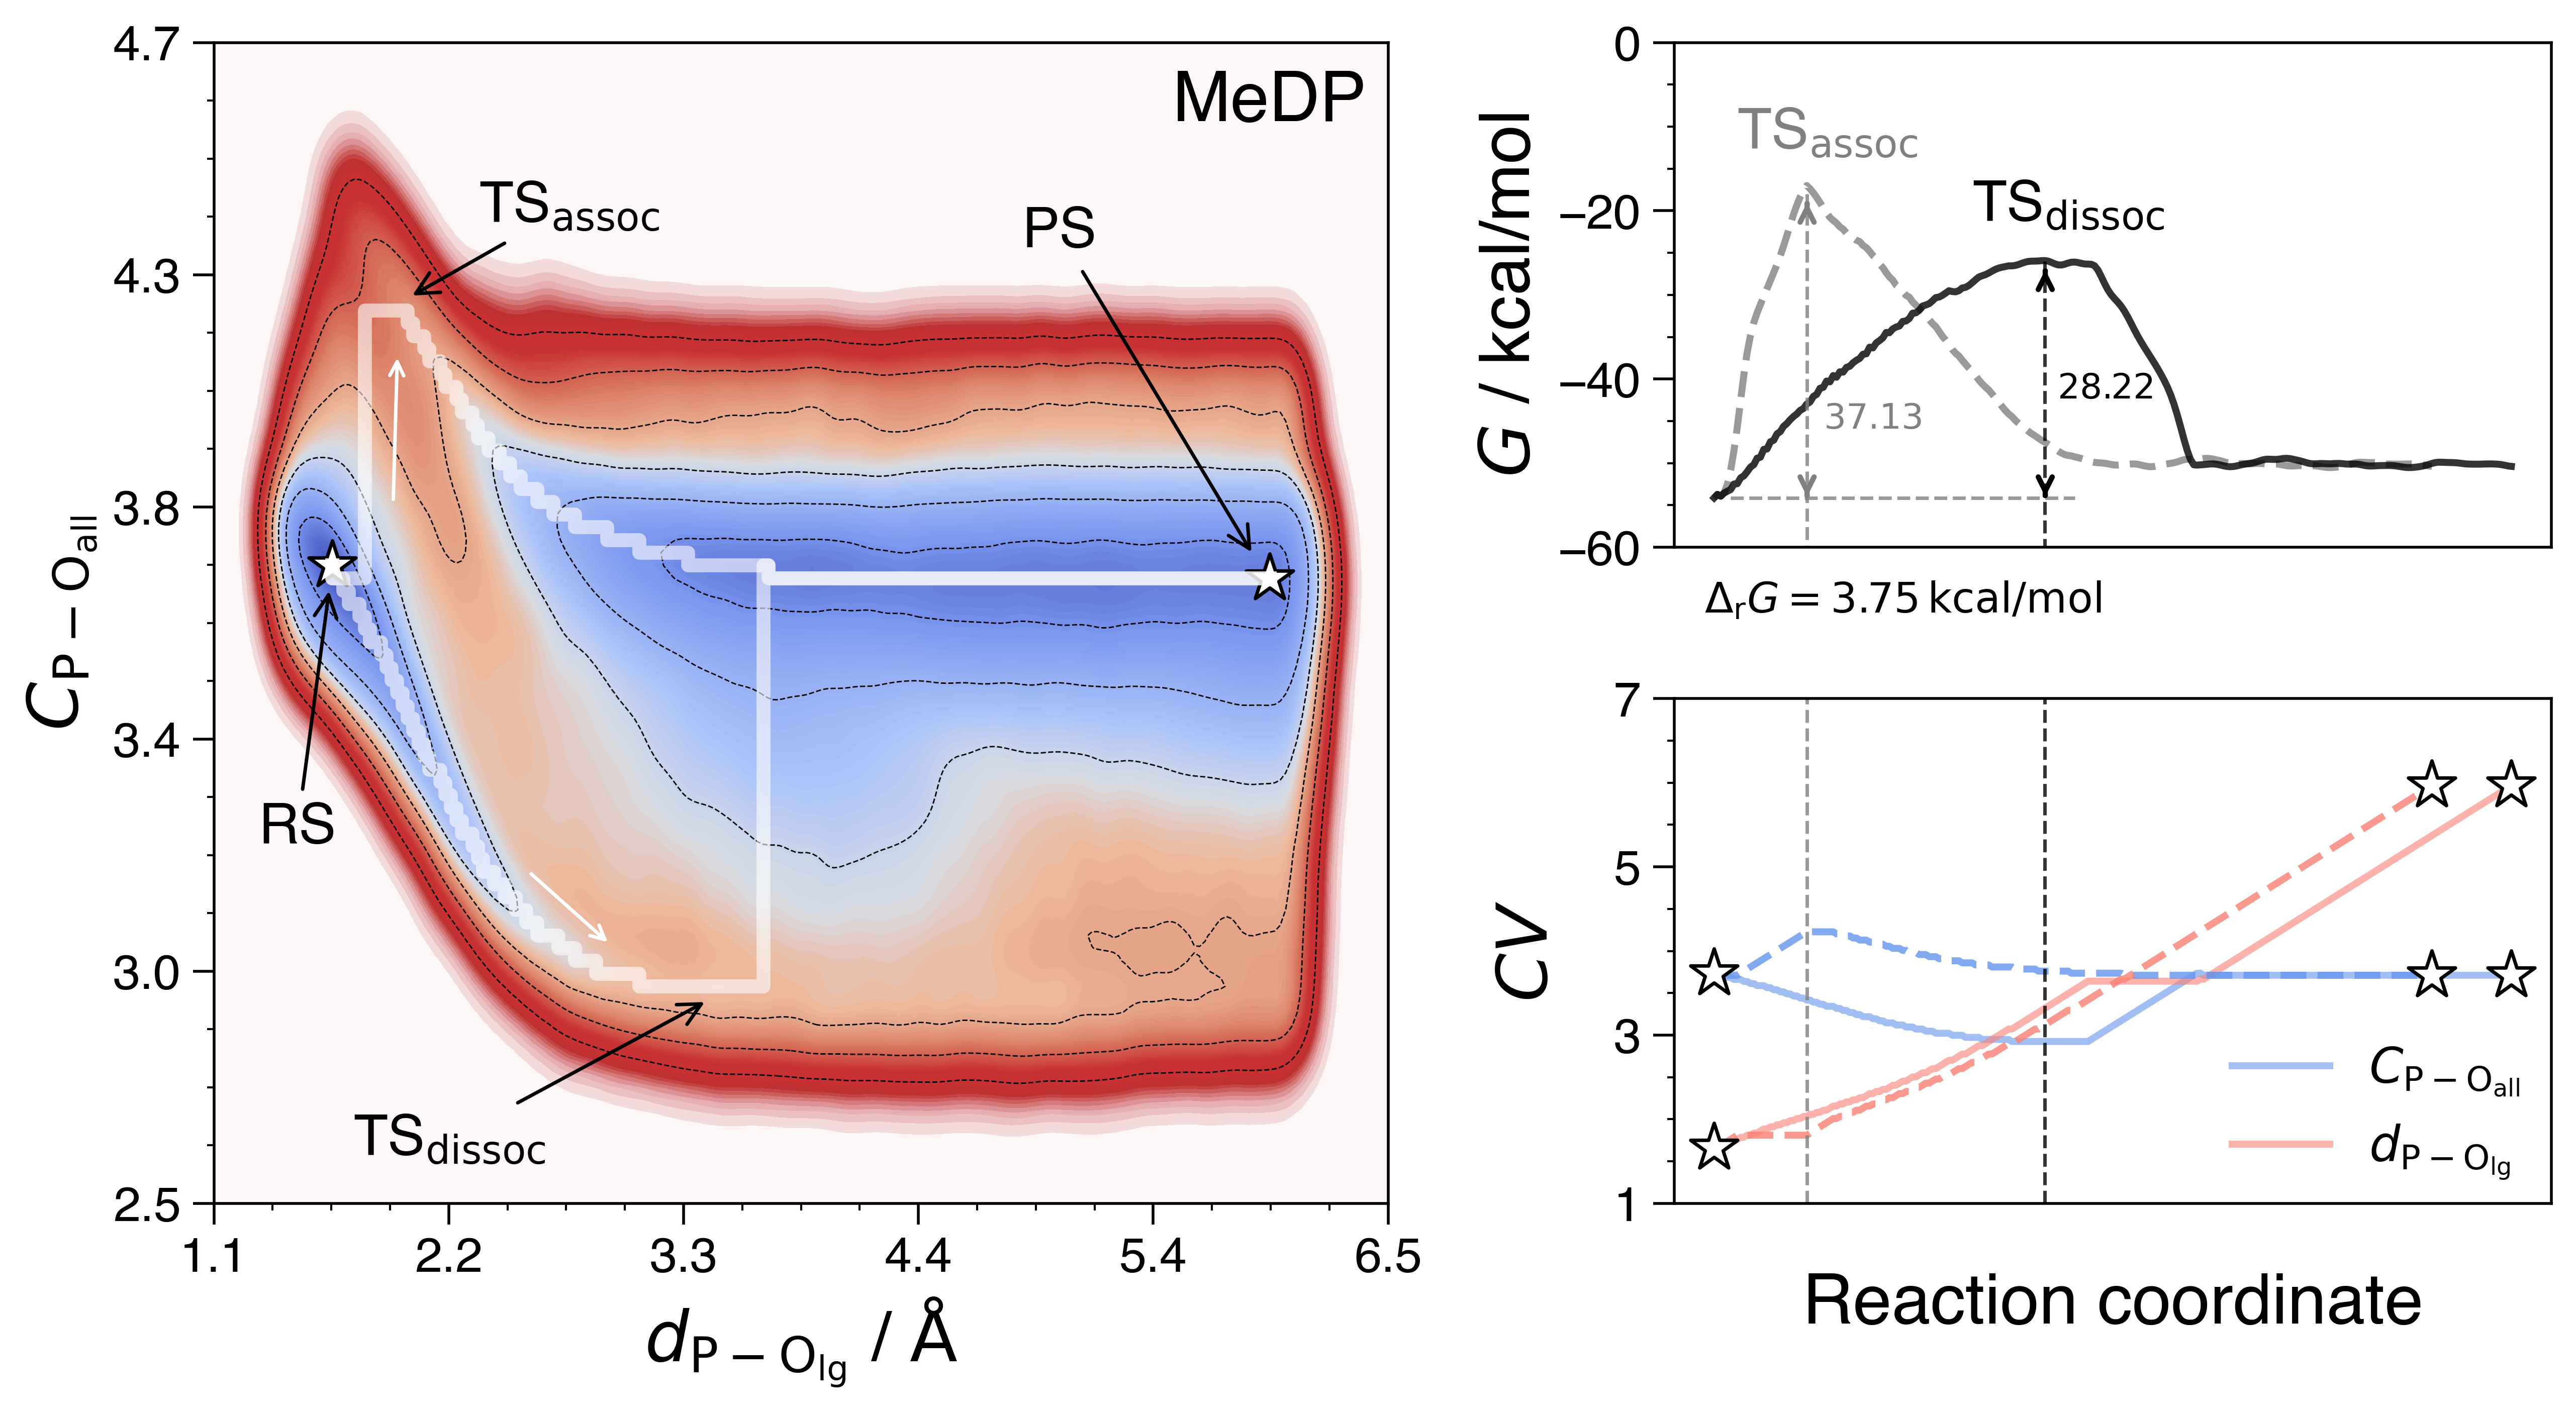
\includegraphics[width=0.85\textwidth]{Figures/4_Results/results_MeDP_300K_fes_mfep.png}
    \caption{(Left panel) \ac{fes} of the \ac{medp} hydrolysis at 300 K, projected on two \acp{cv}, and the corresponding \ac{mfep} with the evolution of the \acp{cv} along the path (right panel).}
    \label{fig:medp_300k_fes_mfep}
\end{figure}

\begin{figure}[ht]
    \centering
    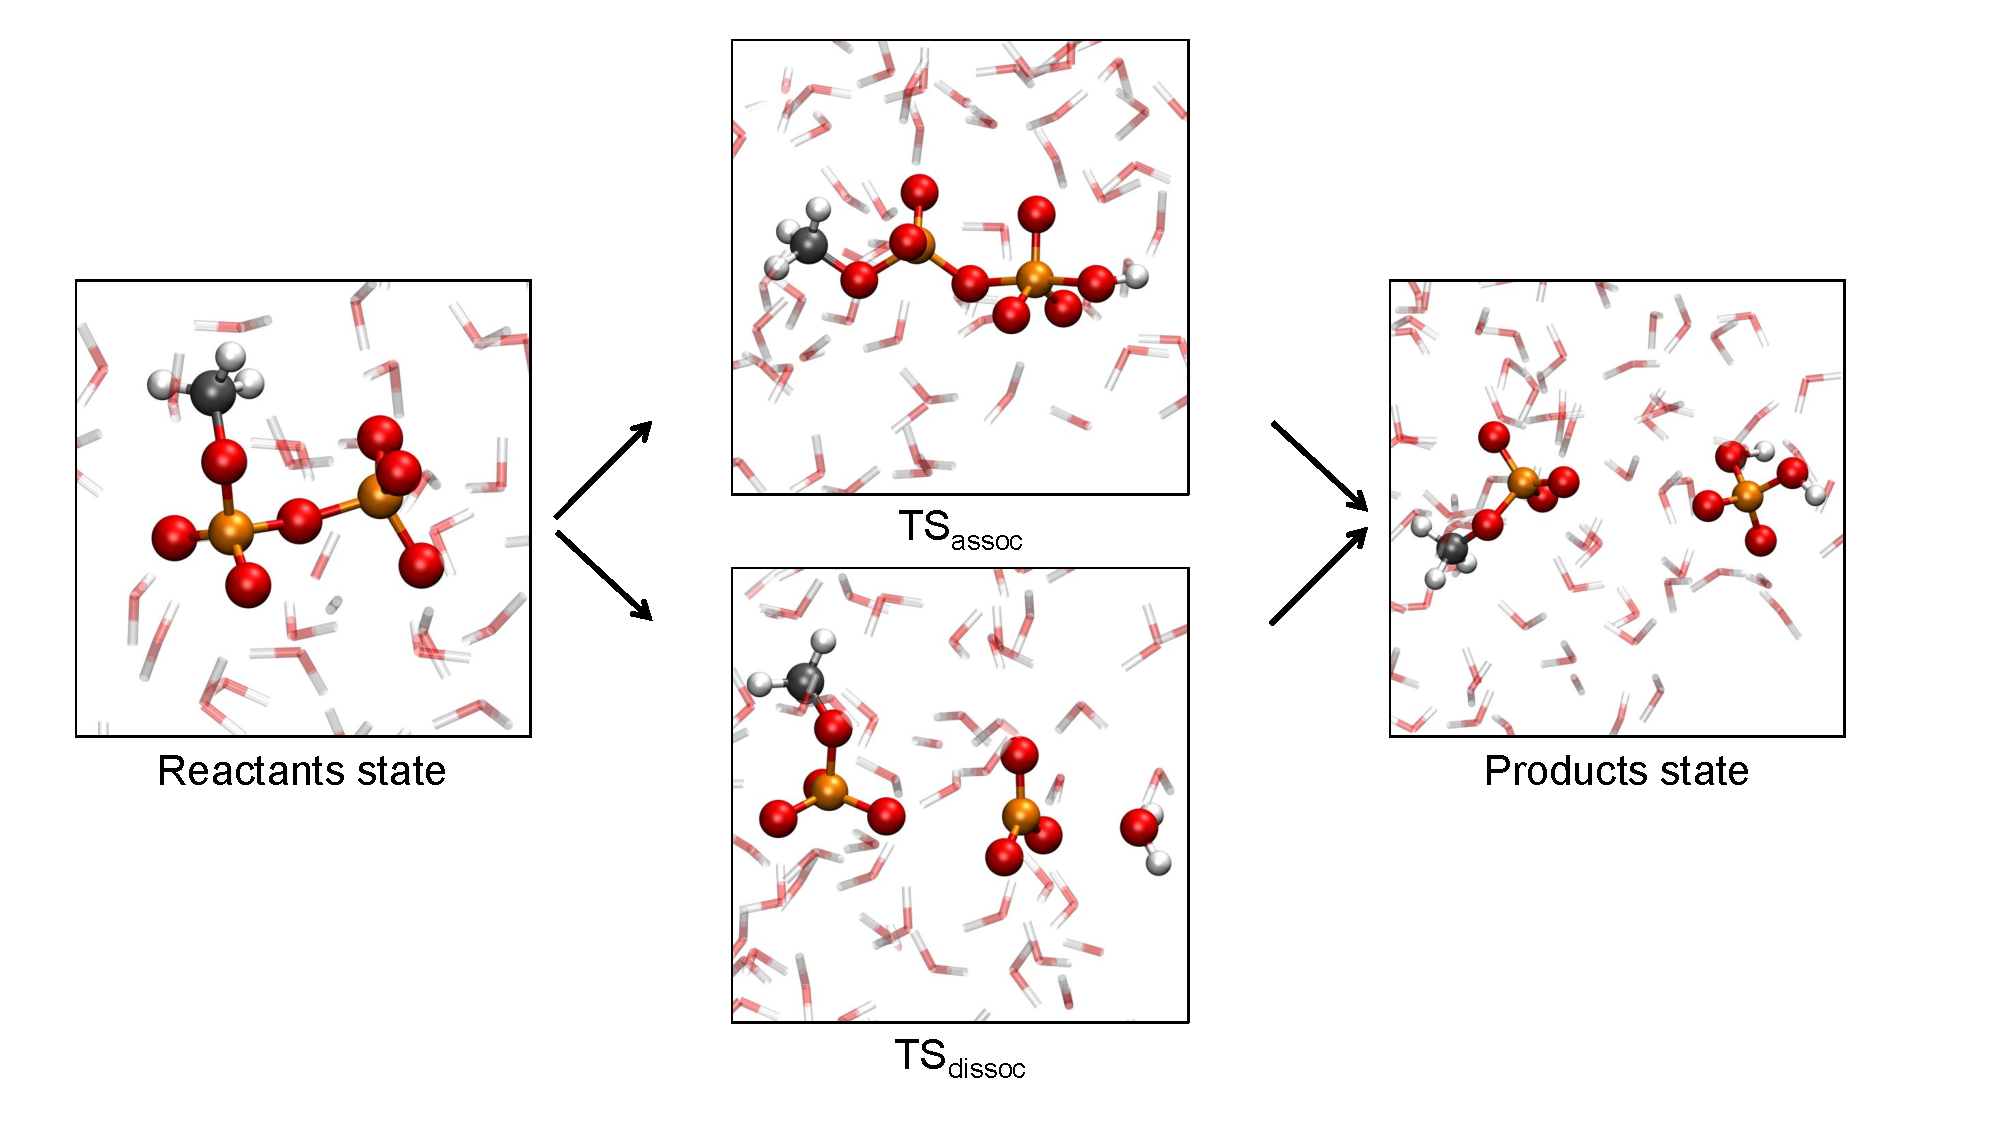
\includegraphics[width=0.85\textwidth]{Figures/4_Results/results_medp_mechanism.pdf}
    \caption{Associative and dissociative reaction pathways for the \ac{medp} hydrolysis with the corresponding reactant, \ac{ts}, and product structures.}
    \label{fig:medp_reaction_mechanism}
\end{figure}

When comparing the two pathways, it is evident that, relative to one another, the dissociative pathway features a late, flatter barrier, while the associative one is early and steeper. To overcome the late barrier of the dissociative route, vibrational energy of the reactants plays a more significant role than translational energy, whereas the opposite is true for the associative pathway~\citep{polanyiConceptsReactionDynamics1987}.

Moreover, the flat profile of the dissociative \ac{ts} suggests the potential existence of a transient intermediate. However, the current \ac{fes} does not provide evidence for such a species. This possibility could be further investigated with longer simulations.

Mechanistically, the dissociative pathway proceeds as follows: the leaving group dissociates from the $\beta$-phosphorus atom, forming a planar metaphosphate species, PO$_3^-$. At this point, the attacking water molecule is still relatively distant ($>2.1$~\AA). Shortly thereafter, a water molecule approaches the $\beta$-phosphorus atom, deprotonates to form a strong nucleophile (OH$^-$), and rapidly forms a bond with the metaphosphate, yielding the product state. Concurrently, the proton is transferred to the newly formed monohydrogen phosphate via the water network in a hopping fashion, following the Grotthuss mechanism~\citep{degrotthussDecompositionLeauCorps1806, cukiermanTuGrotthussOther2006}. This dissociative mechanism is illustrated in Figure~\ref{fig:medp_reaction_mechanism}. Examination of the \ac{mfep} and the \ac{cv} evolution along the path (right panel of Figure~\ref{fig:medp_300k_fes_mfep}) shows that the water attack mainly occurs in the descending region following the flat \ac{ts}. Overall, the dissociative pathway closely resembles the dissociative/concerted D\textsubscript{N}A\textsubscript{N} mechanism (described in detail in Section~\ref{subsec:diphosphates_reaction_mechanism}), which involves departure of the leaving group (D\textsubscript{N}) followed by nucleophilic addition (A\textsubscript{N}) in one step.

In the associative pathway, the mechanism is as follows: the leaving group remains attached to the $\beta$-phosphorus atom while the attacking water molecule approaches. Upon close contact, the water molecule deprotonates and forms a pentacoordinated \ac{ts}. The leaving group then departs, and the proton is transferred to the monohydrogen phosphate via the water network, again following a hopping mechanism. This associative mechanism is also depicted in Figure~\ref{fig:medp_reaction_mechanism}. The \ac{mfep} and \ac{cv} evolution along the pathway (Figure~\ref{fig:medp_300k_fes_mfep}, right panel) show that the maximum in the coordination number aligns closely with the highest point on the \ac{mfep}, consistent with the associative/concerted A\textsubscript{N}D\textsubscript{N} mechanism, which involves nucleophilic addition (A\textsubscript{N}) followed by departure (D\textsubscript{N}) in one step.

The experimentally determined barrier height for \ac{medp} hydrolysis at 25\textdegree{C} (298 K) is 29.2 kcal/mol~\citep{wolfendenDegreesDifficultyWaterConsuming2006}, suggesting that the reaction proceeds via a dissociative/concerted D\textsubscript{N}A\textsubscript{N} mechanism. It is important to note that this conclusion is based on the model chemistry employed in this work: an \ac{nnp} trained on the PBE-D3(BJ)/TZV2P level of theory. This functional is known to have limitations in predicting reaction energies and barrier heights~\citep{burschBestPracticeDFTProtocols2022}, and in accurately describing the structure of bulk water at ambient temperature, as discussed in Section~\ref{sec:water_rdf}. Nevertheless, the long-timescale \ac{aimd} simulations driven by the \ac{nnp} predict a barrier height of 28.22 kcal/mol, which is in good agreement with the experimental value and within both the model’s error margin and the threshold of chemical accuracy. This suggests that the compromise approach adopted in this work is capable of capturing the reaction mechanism and kinetics of phosphate hydrolysis effectively.



%%%%%%%%%%%%%%%%%%%%%%%%%%%%%%%%%%%%%%%%%%%%%%%%%%%%%%%%%%%%%%%%%%%%%%%%%%%%%%%%
\section{Reaction mechanism for methyl diphosphate dianion}

\begin{figure}[b!]
\centering
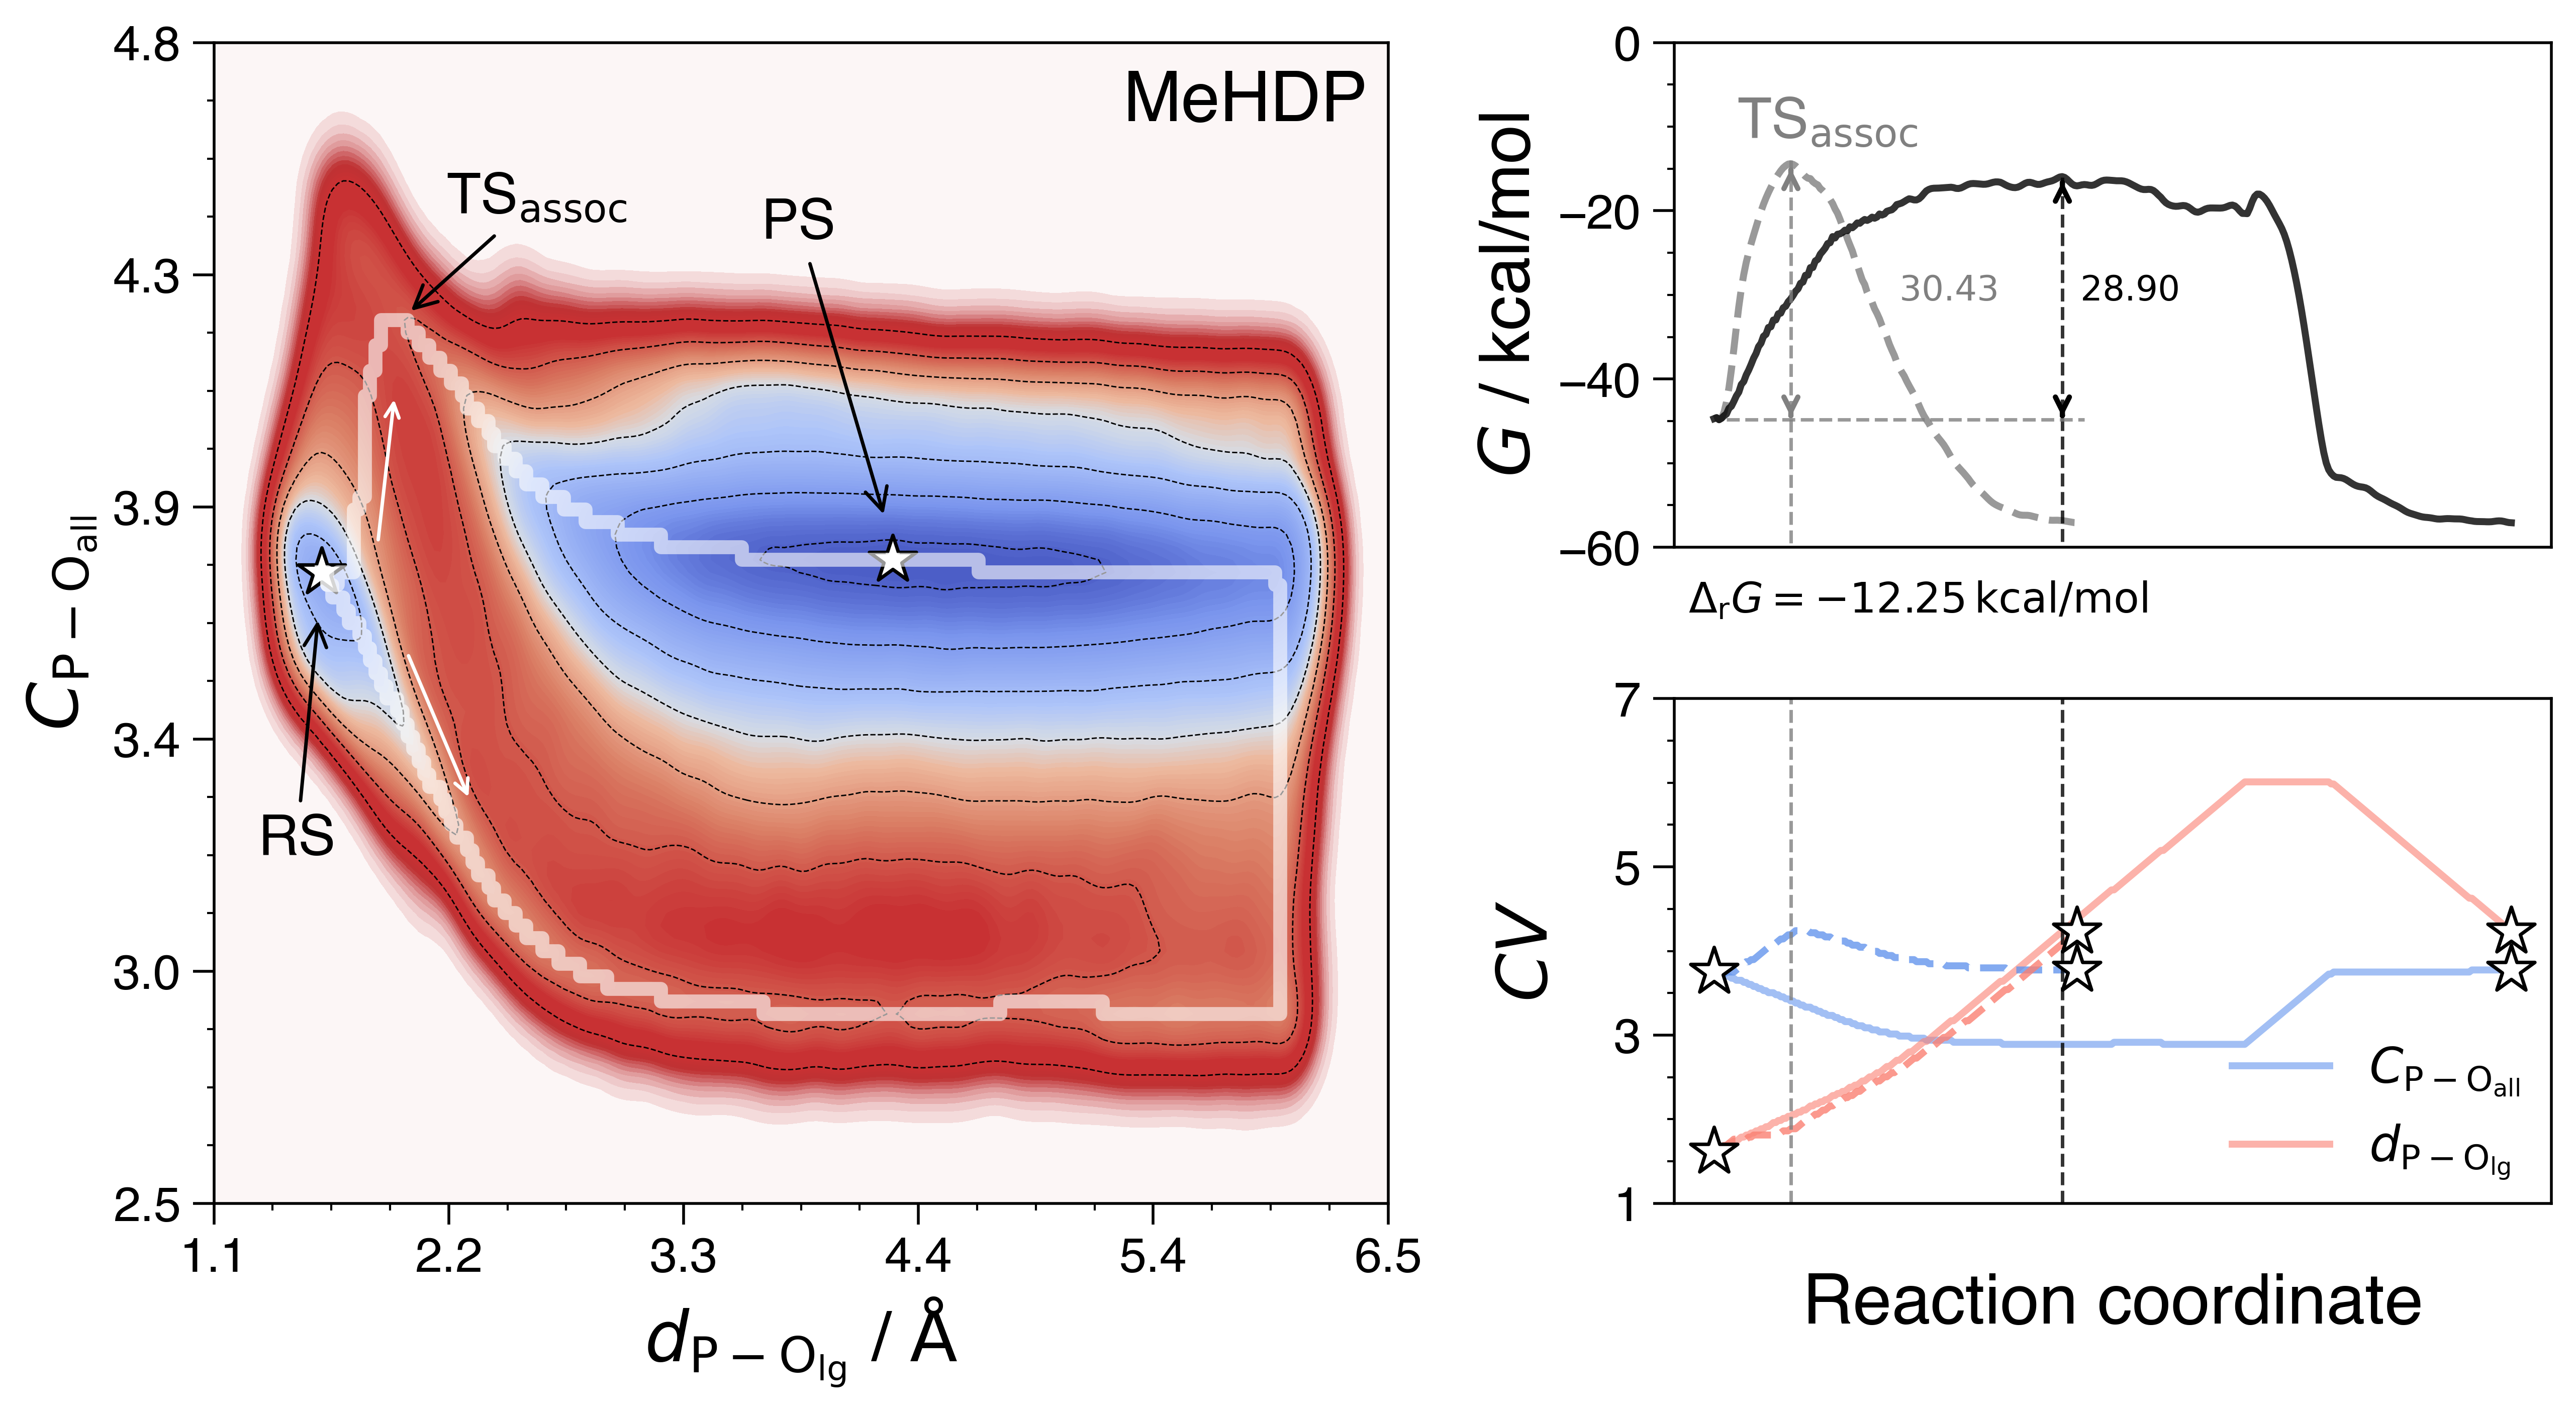
\includegraphics[width=0.85\textwidth]{Figures/4_Results/results_MeHDP_300K_fes_mfep.png}
\caption{(Left panel) \ac{fes} of the \ac{mehdp} hydrolysis at 300 K, projected on two \acp{cv} and the corresponding \ac{mfep} with the evolution of the \acp{cv} along the path (right panel).}
\label{fig:mehdp_300k_fes_mfep}
\end{figure}

Turning to the hydrolysis of the protonated form of \ac{medp}, namely \ac{mehdp}, the corresponding \ac{fes} is shown in Figure~\ref{fig:mehdp_300k_fes_mfep}. The left panel presents the \ac{fes} projected onto two \acp{cv}, while the right panel shows the corresponding \ac{mfep} and the evolution of the \acp{cv} along the path.

In this case, the \ac{fes} appears to be undersampled, as indicated by the flat and broad region along the potential dissociative pathway. In contrast, the associative pathway is better sampled and displays a well-defined \ac{ts} region. The global minimum of the \ac{fes} is located in the products basin. A 3D reconstruction of the \ac{fes} is available in Figure~\ref{fig:fes_3d_mehdp_300k} in the Appendix.

The broad and flat nature of the dissociative pathway suggests the possible existence of an intermediate state that lies higher in energy than both the reactant and product states. This observation, together with the shape of the \ac{mfep}, implies that the hydrolysis mechanisms of \ac{medp} and \ac{mehdp} differ fundamentally. Furthermore, based on the barrier height of the associative pathway, the dissociative route is expected to be more favourable. This hypothesis can be further evaluated through extended \ac{wtmd} simulations.

The associative pathway features a \ac{ts} at a $d_\mathrm{P-O_{\mathrm{lg}}}$ of 1.89~\AA\ and a coordination number of 4.19, which is consistent with the associative \ac{ts} observed for \ac{medp}. This tight \ac{ts} features a pentacoordinated phosphorus atom, as illustrated in Figure~\ref{fig:mehdp_reaction_mechanism}. The associated barrier height is 30.43 kcal/mol, which is notably lower than the 37.13 kcal/mol barrier observed for the associative pathway of \ac{medp} hydrolysis. This observation suggests that \ac{mehdp} is more reactive than the trianion. It further supports the fact that protonation of the phosphate group enhances its reactivity, which can be attributed to the effect of the leaving group's $\mathrm{pK}_\mathrm{a}$.

\begin{figure}[b!]
\centering
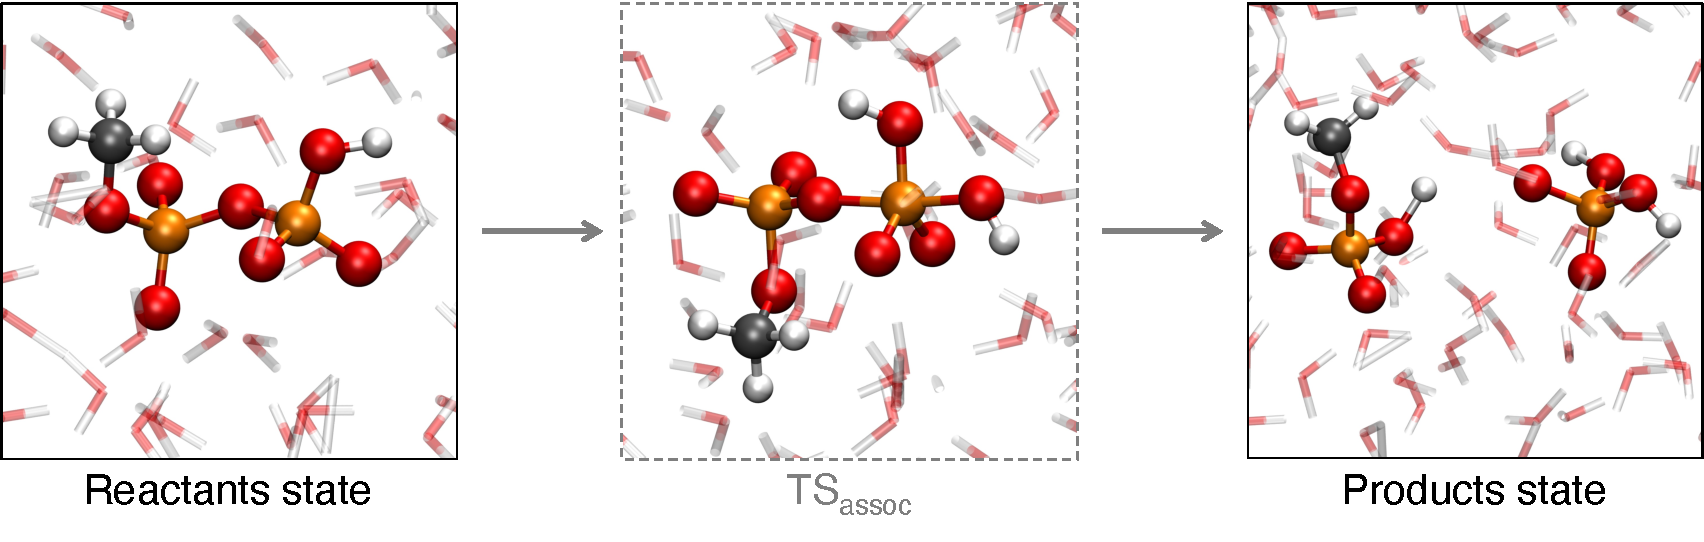
\includegraphics[width=0.85\textwidth]{Figures/4_Results/results_mehdp_mechanism.pdf}
\caption{Associative reaction mechanism of the \ac{mehdp} hydrolysis with the corresponding reactant, \ac{ts}, and product structures.}
\label{fig:mehdp_reaction_mechanism}
\end{figure}

The mechanism of the associative pathway proceeds via the following steps: the leaving group remains attached to the $\beta$-phosphorus atom while the attacking water molecule approaches. Upon close contact, the water molecule deprotonates, forming a tight, pentacoordinated \ac{ts}, analogous to the case of \ac{medp}. In this state, the hydrogen of the terminal group is oriented towards the leaving group. Upon departure of the leaving group, a proton is first transferred from the newly formed dihydrogen phosphate to the leaving group. Shortly thereafter, the monohydrogen phosphate is protonated via the water network, again through a hopping mechanism. The final products are thus formed. This associative mechanism is also illustrated in Figure~\ref{fig:mehdp_reaction_mechanism}. The \ac{mfep} and the evolution of the \acp{cv} along the pathway (right panel of Figure~\ref{fig:mehdp_300k_fes_mfep}) reveal that the maximum in the coordination number aligns closely with the highest point on the \ac{mfep}, which is consistent with the associative/concerted A\textsubscript{N}D\textsubscript{N} mechanism, involving nucleophilic addition (A\textsubscript{N}) followed by nucleophilic departure (D\textsubscript{N}) in a single step.

The experimentally determined barrier height for \ac{mehdp} hydrolysis at 25\textdegree{C} (298 K) is 27.7 kcal/mol~\citep{wolfendenDegreesDifficultyWaterConsuming2006}. To compare the results of this study with the experimental data, further calculations are necessary to obtain a fully converged dissociative pathway, which would allow a more balanced comparison with the associative mechanism.

Finally, it is worth noting that neither the \ac{medp} nor the \ac{mehdp} 3D \ac{fes} (Figures~\ref{fig:fes_3d_medp_300k} and~\ref{fig:fes_3d_mehdp_300k}, respectively) displays a well-defined first-order saddle point. This limitation can be addressed by further converging the \ac{fes}, which would yield smoother surfaces and enable normal mode analysis on the selected points in the \ac{ts} regions to confirm whether they have a single imaginary frequency.



%%%%%%%%%%%%%%%%%%%%%%%%%%%%%%%%%%%%%%%%%%%%%%%%%%%%%%%%%%%%%%%%%%%%%%%%%%%%%%%%

\section{Proton transfer mechanism}

\begin{figure}[b!]
    \centering
    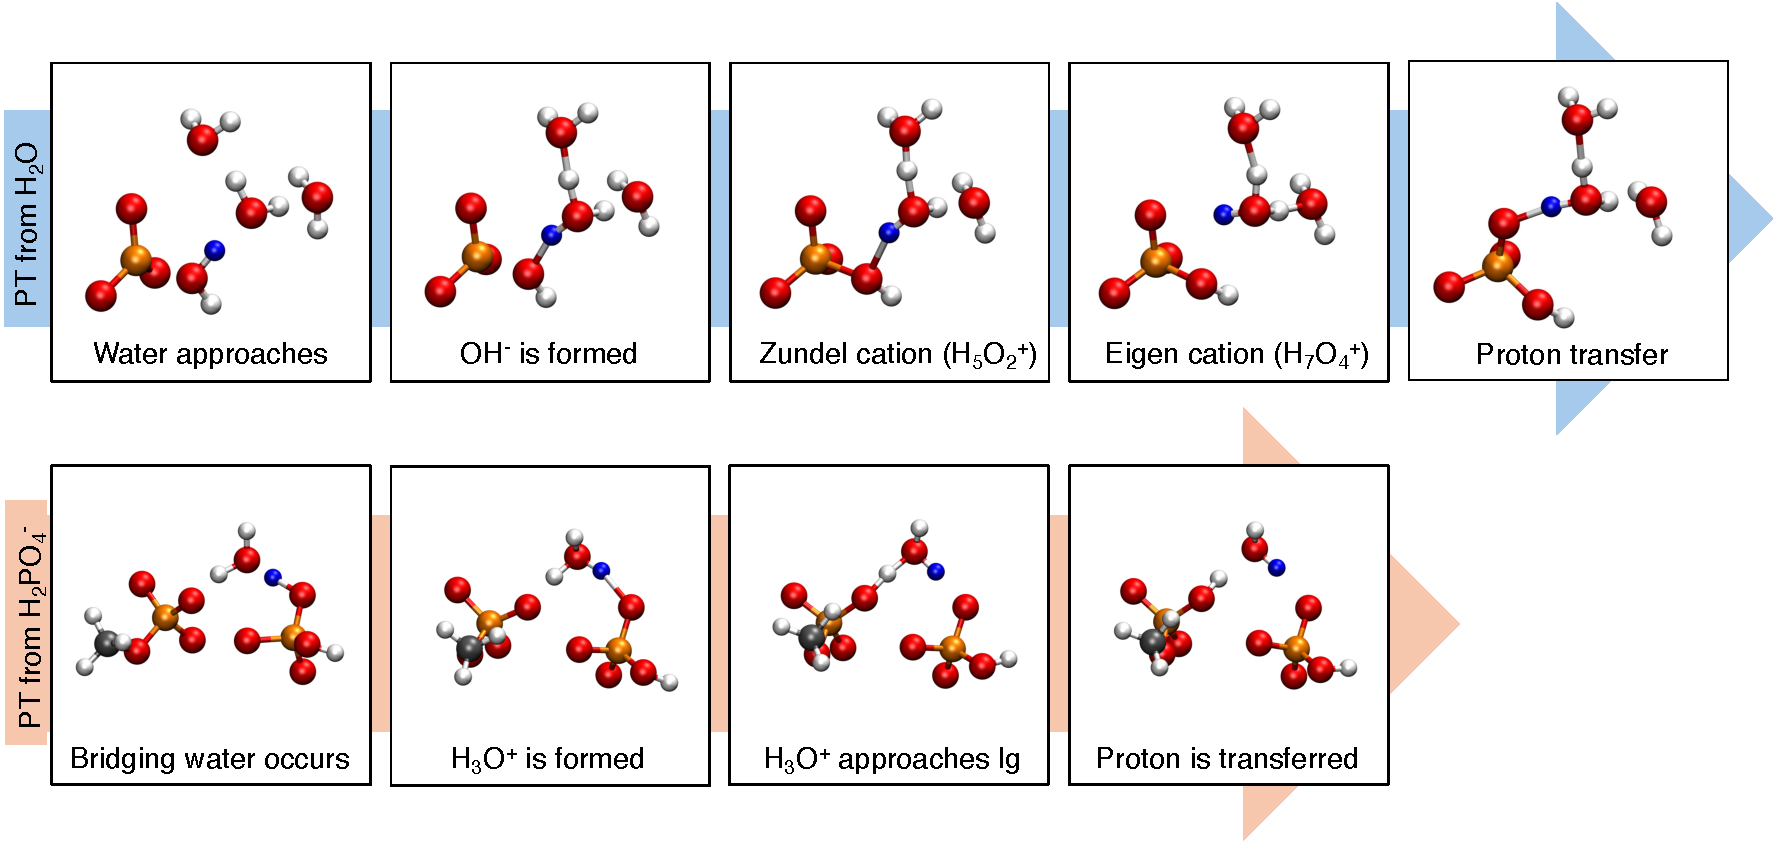
\includegraphics[width=0.85\textwidth]{Figures/4_Results/results_proton_transfer.pdf}
    \caption{\Acf{pt} mechanism depicted step by step from the \ac{medp} D\textsubscript{N}A\textsubscript{N} dissociative mechanism and the \ac{mehdp} A\textsubscript{N}D\textsubscript{N} associative mechanism.}
    \label{fig:medp_proton_transfer}
\end{figure}

We now come to the dessert of this study - the proton transfer mechanism. As in any other study of a chemical reaction carried out using biased sampling, numerous reactive events occur during the simulations. In the production runs conducted in this work, several proton transfer events were observed, although only a few were analysed in detail. Specifically, two types of proton transfer events were identified: one in which a proton is transferred from a water molecule to the PO$_3^-$ species (and possibly to the monohydrogen phosphate), and another in which a proton is transferred from the dihydrogen phosphate to the leaving group. These events are illustrated in Figure~\ref{fig:medp_proton_transfer}.

During the \ac{wtmd} production runs, the \ac{cv} associated with any hydrogen atom in the system was not biased. This implies that the proton transfer events occurred spontaneously.

When the \ac{pt} takes place from a water molecule, it proceeds through the following steps: first, the water molecule approaches the reactive site; then, a neighbouring water molecule from the second solvation shell activates the former by deprotonating it, resulting in the formation of a Zundel complex (H$_5$O$_2^+$)~\citep{xantheasDancesHydrogenCations2009, zundelEnergiebanderTunnelndenUberschussProtonen1968}, which can be described as a proton shared between two water molecules. Subsequently, an Eigen complex (H$_7$O$_3^+$)~\citep{xantheasDancesHydrogenCations2009, eigenProtonTransferAcidBase1964} is formed with the involvement of a third water molecule from the second solvation shell. In this structure, the hydronium ion (H$_3$O$^+$) is typically stabilised by two or three water molecules. The proton is then transferred to the newly formed monohydrogen phosphate.

In the case where the \ac{pt} occurs from the dihydrogen phosphate, the proton is transferred to the leaving group via a bridging water molecule, leading to the formation of the hydronium cation and the consequent proton transfer.

In summary, proton transfer occurs with the assistance of either one or three water molecules. A more detailed analysis of the proton transfer mechanism would be a valuable direction for future work, particularly to determine the average number of water molecules involved in the proton transfer network.
